\documentclass[11pt, oneside]{article}   	
\usepackage[margin = 1 in]{geometry}                		
\geometry{letterpaper}                   		
%\usepackage[parfill]{parskip}    %Begin paragraphs with an empty line rather than an indent
\usepackage{graphicx}				
\usepackage{setspace}								
\usepackage{amssymb}
\doublespacing
%\geometry{footnotesep=2\baselineskip}
\interfootnotelinepenalty=10000 %prevents long footnotes from overflowing to new page
\usepackage{longtable}
\usepackage{caption} %Put caption* in a table to remove the enumeration
\usepackage{rotating} % To rotate the reviewer table
\usepackage{natbib}   %activates bibliography
\usepackage [english]{babel} %something for bibliography
\usepackage{verbatim} %to be able to use \begin{comment}
\usepackage{booktabs}
\usepackage{array}
\usepackage{float} 
\usepackage{pdflscape} %allows for one page to be landscape (lscape makes word landscape, pdflscape makes page landscape)

\begin{document}

% make reviews / time on market a measure
% update intro to match results

\title{Measuring Discrimination: The Impact of Host Race and Gender on Earnings from Airbnb\footnote
	{I thank Steven D. Levitt for valuable advice. Kirthi Bellamkonda, Jacob Dorn, Michal Dzitko, Sonia Jaffe, Ezra Karger, Sylvia Klosin, Victor Lima, and Kotaro Yoshida provided excellent feedback and comments. Mahathi Ayyagari, Fong Chai, Joseph Day, Melody Jih, Spencer Kang, Cristian Raygoza, Thiago Resende, Tony Song, Lydia Sum, Putter Thepkanjana, and Leah Umanskiy provided research assistance. All remaining errors are my own. Data was provided by InsideAirbnb.com, founded and maintained by Murray Cox. Airbnb was not consulted in this research. Sentiment analysis would not be possible without Sentimentr and coding by Ben Chaimberg.}}
\author{Anya Marchenko\footnote{University of Chicago, Becker Friedman Institute}}
\maketitle

\begin{abstract}
This paper leverages the recent rise of sharing economies and the standardization of their platforms to credibly measure discrimination against minority landlords on Airbnb. Using a previously unexploited dataset created by scraping the Airbnb website, I estimate that black hosts earn \$5 - \$7 less per night and Asian hosts \$6 - \$9 less per night (depending on the sex of the host) than white hosts who post a similar type of listing. Crucially, I use two measures of quantity demanded of hosts' listings to estimate whether a demand or supply shift is responsible for the price disparity. I find that despite their lower prices, black hosts face lower demand. This is consistent with the presence of discrimination. 
\\\\
\textit{Keywords}: Prejudice and Bias; Online Technology; Race; Trust; Renting or Rental; Accommodations Industry; Real Estate Industry

\end{abstract}

\newpage

\doublespacing
\section{Introduction}

African-Americans have experienced pervasively worse outcomes in the housing market, and historic and current racial discrimination is one major cause.\cite{krysan} Even after the gains of the Civil Rights Era, such as the landmark Fair Housing Act of 1968, discrimination in the housing market is widely documented by social scientists. Yinger (1986) measured discrimination using fair housing audits and found that black renters are told that there are 30\% fewer available housing units than white renters.\cite{Yinger, John. "Measuring racial discrimination with fair housing audits: Caught in the act." The American Economic Review (1986): 881-893.} African-American families face higher barriers when raising capital to purchase a home, since black applicants get fewer loans for the same application as white applicants.\cite{pope} [EXAMPLE 3]. Landlords renting out apartments discriminate both because of their own prejudice and in response to the prejudice of their white renters.%
	\footnote{Some studies have found evidence that discrimination in rental markets is statistical in nature (that is, landlords use race as a proxy for income). For African-Americans who imply that they are of a higher social class when applying for an apartment, discrimination is virtually not present.\cite{Hanson, Andrew, and Zackary Hawley. "Do landlords discriminate in the rental housing market? Evidence from an internet field experiment in US cities." Journal of Urban Economics 70.2 (2011): 99-114.}}
\cite{Ondrich, Jan, Alex Stricker, and John Yinger. "Do landlords discriminate? The incidence and causes of racial discrimination in rental housing markets." Journal of Housing Economics 8.3 (1999): 185-204.}

Economists have primarily studied discrimination against African-American tenants. There is little research on the other side of the market - when African-Americans are supplying, rather than demanding, housing.%
	\footnote{One would also expect black landlords to fare worse than white landlords in this area as well. Properties owned by African-Americans tend to be less expensive than those owned by white Americans. The average black household still has less mean wealth than a white household.\cite{oliver} Even middle-class black and Hispanic households still live in neighborhoods with median incomes similar to those of very poor white neighborhoods.\cite{reardon}} 
Logistically, it is difficult for researchers to conduct an experiment to randomize ownership of property to landlords of different races. Without randomization, it is difficult to disentangle true discrimination from systematic differences in the housing owned by African-Americans and white landlords. **INSERT 'BAD' LANDLORD STUDIES HERE**. Some studies have found anecdotal evidence of discrimination against African-American landlords. 

This paper leverages the recent rise of sharing economies and the data and standardization their platforms provide to credibly measure discrimination against minority landlords. Airbnb is a sharing economy platform that allows people to rent out their apartment, house, or single room to short-term lodgers. Since Airbnb simply provides an online platform for a market that already exists, it is reasonable to assume that agents will discriminate on Airbnb in a similar way that they discriminate in the real world. This means that studying discrimination in sharing economies could be an important way to learn about discrimination in traditional housing markets as well.
%Sharing economies are convenient for research in several distinct ways. First, all agents on the platform obey a uniform set of rules and observe the same set of information about one another. Second, sharing economies allow for cleaner data collection, as well as both price and a proxy for quantity demand for each listing. 

Measurements of discrimination on Airbnb are still potentially confounded by many other factors that affect a listing's price. Edelman and Luca (2014) estimated the effect of host race on the price of their listing in New York City with a small set of controls. Their results suggest that non-black hosts on Airbnb have prices roughly 12\% higher than black hosts. However, they control for only a few property characteristics, the quality of the host's reviews, and a measure of the reliability of the host. They leave out many other unobservables that could be confounding the effect such as the location of the listing (an important factor, especially in New York), the type of listing (which can vary from a single room to an entire house), and proxies for the quality of the host themselves. %CHECK WHETHER THEY ACTUALLY LEFT OUT LOCATION

In this paper, I use a new, previously unexploited dataset from a webscrape of Airbnb to empirically measure discrimination. Using price and listing information for 70,000 Airbnb hosts throughout the country, I address the limitations of Edelman and Luca's research by controlling for location, additional property characteristics, comprehensive measures of listing size, and text analyses of host-written descriptions of the listing. 

Crucially, the data allows for estimation of not just the price, but the vacancy rate of a listing, which is a measure of the quantity demanded. Knowing both quantity and price allows me to distinguish whether the price disparity between minority and white hosts on Airbnb is due to a demand shift (consistent with discrimination) or a supply shift (consistent with a difference in marginal cost for the hosts, or other hypothesis, discussed below). 

I find that non-white hosts, both male and female, have lower prices than white hosts. The biggest effect is for Asian female hosts, whose prices are roughly \$9 less per day than white male hosts who own the same type of listing. The second biggest effect is for black males, with a coefficient of \$7, followed by black women and Asian men with coefficients of \$6 per day, and Hispanic females with a coefficient of \$5.%
	\footnote{This effect is statistically significant at the p $<$ .001 level for black hosts and Asian women, the p $<$ .01 level for Asian male hosts, and p $<$ .05 level for Hispanic women.} 
For Hispanic men the effect is small, around \$2, and is not statistically significant.

My coefficients are smaller than Edelman and Luca's, raising the concern that the price disparity measured could be erased altogether by adding more controls. I attempt to address this problem by adding measures of host quality and listing attractiveness that could differentiate one listing from another for a given property size and type. I find that the price disparity is stable to the addition of these controls, providing confidence that adding more variables of a similar nature would not eliminate the disparity. 

After having addressed the empirical robustness of this main finding, I test several alternative hypotheses that could explain the price disparity. In contrast to previous research, my data on the vacancy rate allows me to distinguish between discrimination and several other mechanisms which could be causing the price disparity. 

One alternative hypothesis for the price disparity is that minority hosts charge a lower price for their listing because it is cheaper for them, on the margin, to operate the same listing as compared to a white host. Since Black and Hispanic workers tend to earn less than their white counterparts, even for the same amount of education, they may have a lower opportunity cost of time.\cite{Economic Policy Institute, State of Working America Data Library, ?Wages by education,? 2016.} Minority hosts would therefore have a lower marginal cost of managing their listing, and so would choose to set lower prices for their listings than white hosts with comparable listings. If the price disparity was due to supply differences, then basic supply and demand theory predicts that the quantity demanded of minority hosts' listings should be higher than white hosts'. To test this hypothesis, I consider the number of reviews that a host has as a proxy for the quantity demanded of that listing. I regress the number of reviews on host race, controlling for the preferred specification. I find that minority hosts have a lower, not higher, number of reviews than white hosts, suggesting that this hypothesis fails to explain the price disparity.%
	\footnote{Throughout this analysis, I assume that guests review hosts of different race at equal rates. X and Y have found that rates of review tend to be the same/different across hosts. MELODY - FIND WHETHER WHETHER THERE'S LIT ON DIFFERENT REVIEW RATES ACROSS RACES. However, if reviewers systematically under-review minority hosts, this itself could be evidence of discrimination. For more discussion on this assumption, see Section 5, Part 1.} 

One potential explanation for their lower number of reviews is that minority hosts make their listing available to guests less frequently than white hosts. A host controls how many days of the month they offer their listing for rent via an availability calendar on the listing page. When a guest books their listing, the booked days disappear from the availability calendar. Therefore, the measure of availability is actually a measure of true vacancy for the listing. If minority hosts have lower numbers of reviews, perhaps this is because they offer their listing for fewer days of the month than white hosts. To test this, I regress a listing's availability out of 30 days on host race, controlling for the preferred specification. Contrary to this hypothesis, regression results show that the listings of black hosts stay vacant 1 - 2 days per month longer than the listings of white hosts. However, there is evidence that Asian hosts do choose to make their listings available less frequently, which would contribute to their lower number of reviews. 

A final, alternative, hypothesis that could account for the price disparity between minority and white hosts is that minority hosts own listings of worse quality, or are simply worse hosts. I consider the quality of a host's reviews as a proxy for the quality of the listing and host. I use the race and gender of the reviewer and the host to compare the sentiment (how favorable or unfavorable the review is) of the reviews that guests leave for white and for minority hosts.%
	\footnote{Since it required hand-coding, demographic information of the reviewers is only available for a randomly-chosen subset of hosts in Chicago.} 
Rather than observing that all minority hosts uniformly had lower quality reviews, which the hypothesis would predict, the significance of the result was either negligible, or depended on the demographics of the reviewer and host. While there is some evidence that male reviewers tend to rate male hosts higher, there is little within-race preference between reviewers and hosts. Taken as a whole, sentiment analysis suggests that minority hosts do not have lower quality reviews. 

\subsection{About Airbnb} 
Airbnb is an online marketplace founded in 2008 that allows hosts to rent their private dwellings to guests as temporary accommodation. As of 2017, it has more than 3 million listings, more than Marriott's 1.2 million rooms worldwide.\cite{aboutus} Just like traditional hotel chains, guests on Airbnb can browse listings by city and property type, and book a stay based on prices, location, past reviews, pictures of the listing, size, and amenities. Unlike traditional hotel chains, however, hosts create a profile for themselves and a page for each listing they are renting. Each listing page includes the name and picture of the host, the reviews left by previous guests, and those guests' profile pictures. Guests can therefore infer demographic information about the host through a host's picture and name, creating the opportunity for discrimination. Figures 1-5 present screenshots of a listing in a Chicago neighborhood, illustrating some of the information that would be available to a potential guest. 


\subsection{Previous Literature} 
Most relevant to this paper is Edelman and Luca (2014), the first paper to identify and measure the extent of anti-host discrimination on Airbnb.\cite{edelman} They explore the effect of host race on the price of their listing using a snapshot of roughly 3,800 New York City hosts in 2012. Controlling for several confounders that influence price, their findings indicate that non-black hosts on Airbnb have prices roughly 12\% higher than black hosts. I build on Edelman and Luca's research in several important ways. First, their sample was relatively narrow and confined to a single city. My sample includes seven cities throughout America, which are all large urban centers, picked so that they cover most geographic regions in the US. It is important to have this variety because discrimination in a large, cosmopolitan city with a highly diverse population such as New York might look different from discrimination in Nashville, which is more racially homogenous.%
	\footnote{According to the U.S. Census Bureau's QuickFacts, Nashvile is 60.4\% white, 28.4\% black, 10.0\% Hispanic, and 2.5\% Asian. New York City is 44\% white, 25.5\% black, 12.7\% Asian, and 28.6\% Hispanic.} 
Second, their set of controls was limited by the relatively sparse listing information available on the Airbnb website (Airbnb has added more comprehensive data on each listing page since 2013). Their covariates only included a listing's location, the number of people the listing accommodates, the rating, the number of bedrooms, and whether or not the whole apartment is available to the guest. After confirming their result when I run a regression using their controls, I then control for a more complete set of covariates (see Section 2.1 and Section 3.1).%
	\footnote{See Table 4 for the results of my regression using their covariates. See Section 3.1 for a discussion of my controls.} 
Most importantly, I also test alternative hypotheses for these price disparities, which Edelman and Luca are unable to address. 

Becker (1957) proposed the idea that discrimination against a group can be reflected in that group's market prices.\cite{becker} In the Airbnb market, Becker's market discrimination would be reflected in the price that the guest (buyer) pays to the host (seller) to stay with them. If the guest (buyer) is discriminating, then given two comparable listings, they would choose not to stay in the one owned by a minority host (seller). Responding to the lower demand, hosts in minority groups rationally post a lower price in a competitive market. 

Becker (1957) was concerned with discrimination arising from face-to-face interactions between minority and majority groups. Since then, there has been a large amount of research indicating that Becker's theory holds for people participating in online labor, lending, rental, and other markets as well. In these cases, participants simply bring their prejudices online and use names and photos to discriminate. A canonical example is the Bertrand and Mullainathan (2004) study, which found that resumes with white sounding names received 50\% more callbacks from potential employers than identical resumes with African-American sounding names.\cite{bertrand} Doleac and Stein (2010) examined market outcomes when selling an iPod on various online marketplaces. In some pictures, a dark-skinned hand was holding the iPod, signaling a black seller, while in others, a light-skinned hand was holding the iPod, signaling a white seller.\cite{doleac} Hands which indicates a black seller received fewer and lower offers than white sellers. In sharing economies, a similar pattern occurs. Uber riders with distinctively African-American names experience longer wait times and more frequent cancellations than riders who use distinctively white names.\cite{knittel} A later study by Edelman and Luca (2016) found a similar result: guests with distinctively African-American names receive 16\% fewer responses from Airbnb hosts than those with white names.\cite{edelman2} These examples suggest that users of online platforms transfer their biases from the real world into the online world.  

\citealp{sharing} 


\begin{comment}
Structurally, African-Americans were denied Federal Housing Adminstration mortgages at the low interest rates that were offered to white families, redlining districts , predatory , among many other structural moving north during the Great Migration were met with  Shut out from One reason is  
Many efforts have been made to curb discrimination in the housing sector against African-Americans. Landmark federal legislation such as the Fair Housing Act of 1968 prohibits housing discrimination based on race, the enforcement of anti-discrimination legislation is difficult on the local level. Residential preferences, differences in family structure and availability of affordable housing contribute to these disparities. Discrimination in housing has also been cited as one of the primary causes of these inequities. 

%Even though the accurate identification and measurement of discrimination by social scientists is vital to creating policies and statutes to combat it, measuring discrimination is difficult. Unobservable variables in the error term make it hard to isolate the effect of discrimination on the outcome variable of interest. Audit studies are one way that researchers can isolate the effect of race, sex, or other demographic on the outcome of interest. However, these types of experiments are not always possible due to the large organizational, manpower, or time costs associated with them. In the absence of an experimental set-up, regression models with a carefully chosen set of controls can aid in the accurate measurement of discrimination.  
Discrimination is difficult to measure. In the real world. Economists and other social scientists have long been concerned with the fact that minorities, especially African-Americans, have experienced pervasively lower living standards in the United States. One potential cause of this is discrimination in the housing market. 

Moreover, many small players have entered these markets who would have otherwise been unable to participate in traditional markets. Managing a room or home with Airbnb has much lower barriers to entry than being the landlord of a large apartment building. In just the 10 years since its founding, Airbnb has surpassed Marriott nearly three-fold in the number of rooms offered worldwide.\cite{sharing} 
\end{comment}

%As more people have entered these new markets, they have become increasingly dependent on the supplementary income they provide. Hosting with Airbnb, a platform that allows people to rent out their apartment, house, or single room to short-term lodgers, is one such opportunity. A 2017 report released by Airbnb states that in rural areas, hosts get as much as 5 - 20\% of their income from their listing.\cite{rural} Airbnb's fastest growing demographic of hosts, women over 60 years of age, earn \$6,000 a year on average from hosting, often relying on that income to supplement retirement savings.\cite{elderly}\cite{nyt2} 

%Some residents of areas of New York City have started relying on hosting with Airbnb to pay for rent or fund retirement. \cite{nyt1} 

%The extent to which hosts have grown to rely on Airbnb as a source of income makes discrimination on the platform a relevant topic of research. The economic consequences of discrimination are substantial - hosts who are discriminated against would face lower demand, have higher vacancies, and earn less revenue from their listing. While one previous paper found evidence of discrimination against New York City hosts using data from 2013, no other more recent or comprehensive research has been done on this type of discrimination on Airbnb. 

%In this paper, I empirically investigate the existence and extent of anti-host discrimination in Airbnb. I start by measuring the effect of host race and sex on the price of the listing and on a constructed measure of host revenue. I use data from a webscrape of around 70,000 Airbnb listings across 7 U.S. cities.\footnote{The scrape includes all of the property, host, and review information on a listing profile. To see what information would be available, see Figures 1-5 for screenshots of a sample listing. All of the information seen on the sample listing is included as variables in the data set.} For each of the 70,000 listings, the race, sex, and age of the host from their profile picture was coded. 

%Next, I construct a measure of host revenue by multiplying the price a host charges by the total number of reviews for that listing (a proxy for the quantity demanded). Using this measure of revenue, I estimate that White female hosts, Black male hosts, Black female hosts, and Asian female hosts lose about \$100-\$300 in revenue over the course of a year as compared to White male hosts who own similar listings. The exact revenue loss depends on the coefficients on price and number of reviews of a particular host.\footnote{See Table 5 and Section 3.2 for the exact effects on revenue.} These effects are statistically significant at the p $<$ .05 level or higher, and significant at the p $<$ .001 level for White females and Black females. There are also negative effects on revenue for Hispanic hosts and Asian males, but they are not significant. In Section 4, I also conduct several robustness checks and show that these results hold across various cities, price ranges, time on the market, and property types.\footnote{See Tables 6, 7 and discussion in Section 4.}

% discrimination is hard to measure, 
% Understanding discrimination in this new housing market is important because it ties into racial discrepancies in housing widely observed by economists and other social scientists. 

% However, it is difficult to separate the effect of current racial discrimination from the confounding effect of these other economic realities. It is therefore unclear to what extent current discrimination, especially in the housing market, contributes to these long-standing economic disparities. 

%Even though the accurate identification and measurement of discrimination by social scientists is vital to creating policies and statutes to combat it, measuring discrimination is difficult. Unobservable variables in the error term make it hard to isolate the effect of discrimination on the outcome variable of interest. Audit studies are one way that researchers can isolate the effect of race, sex, or other demographic on the outcome of interest. However, these types of experiments are not always possible due to the large organizational, manpower, or time costs associated with them. In the absence of an experimental set-up, regression models with a carefully chosen set of controls can aid in the accurate measurement of discrimination.  

% Economists and other social scientists have long documented the poor housing outcomes for minorities, particularly African-Americans, in the housing market.
	\label{lit}
	
\section{Data}
\subsection{Source} 

My data are taken from the website Inside Airbnb, which provides cleaned and aggregated data on Airbnb listings in 43 cities across the world.\cite{insideairbnb} The data provided on the website are sourced from a webscrape of publicly available information on the Airbnb website. Inside Airbnb is not run by or affiliated with Airbnb itself.%
	\footnote{Airbnb's host profiles and listings are publicly available information, and no private data was accessed in the scrape. The cleaned data is under a Creative Commons Public Domain Dedication.} 
The intent of Inside Airbnb is to inform the public on how Airbnb competes with the residential housing market in their areas. 

The scrape of the Airbnb website was conducted throughout 2015, and provides a point-in-time snapshot of all of the listings available in a particular city. This includes all of the information that would be available to an Airbnb user browsing through listings at the time of the scrape. 

A total of 70,000 host pictures across seven US cities were coded - Chicago, Los Angeles, New York City, Austin, Washington, D.C., and New Orleans.%
	\footnote{For every city but New York, every single Airbnb listing that existed in that city at the time of the scrape was coded. In New York, which had the most listings in the sample, half of the existing 40,000 listings were randomly chosen to be coded. Time, effort, and monetary constraints prohibited the coding of all 16 US cities whose data was available on InsideAirbnb.com.} 
Large cities with racial diversity which were geographically dispersed were chosen. This approach limits the applicability of my findings to urban areas, discounting the roughly fifth of Airbnb's listings which are located in rural areas.%
	\footnote{A 2017 report released by Airbnb stated that 18.4\% of all active listings are located in rural areas, and there was 138\% year-in-year growth in Airbnb guest arrivals at rural listings.} 
In addition to main host data, demographic data was also coded for 16,000 reviewers who stayed with a subset of the Chicago hosts.%
	\footnote{This represents about 23\% of the total number of reviewers in Chicago. Not all reviewers could be coded due to time and manpower constraints. A random subset of Chicago hosts was chosen such that the 16,000 reviews represent all of the reviews left for those hosts. Each review has a unique reviewer id, host id, listing id, the date of the review, the review text, and the coded race, sex, and age of the reviewer.}
For those hosts in Chicago, it is thus possible to study the interaction of reviewer demographics, host demographics, and review quality.


\subsection{Data Summary}

Summary statistics of host demographic information and their listings are displayed in Table 2. There is significant variation in both sex and race of the hosts on Airbnb. Roughly a third of the sample are single females, and a third are single males, with the rest being couples or groups.%
	\footnote{38\% of the sample are single females, 31\% are single males, 23\% are couples, and the other 8\% are groups $>$ 2 or pictures without a face. Couples and other groups were not included in the final analysis.} 
About two-thirds of the hosts are white (X\%) MELODY - INSERT REAL PERCENTAGES HERE FROM THE SUMMARY TABLE, and less than a tenth are black (X\%), Hispanic (X\%), or Asian hosts (X\%).%
	\footnote{64\% of the hosts in the sample are white, 7\% are black, 5\% are Hispanic, and 9\% are Asian. The rest of the profile pictures were either pictures of groups, pictures without a human face, or multiracial couples, all of which were put in the ``Unknown/Multiracial" category in Table 2.} 
Black hosts in the sample are underrepresented relative to the proportion of African-Americans in the national population (13\%). Hispanic hosts are similarly very underrepresented relative to the proportion of Hispanics in the population (16\%). One explanation for this could be that people self-identify as Hispanic for census data, while Airbnb hosts were identified by RAs who might have mistakenly coded Hispanic hosts as other categories. Asian-American hosts (X\%) are overrepresented by a few percentage points relative to the 5.6\% of Asian-Americans in the national average.\cite{census} 

The prices of listings owned by white hosts are dramatically higher than those of other hosts. The mean price per night of a listing is \$178 for white hosts, down to \$125 per night for black hosts, \$160 per night for Hispanic hosts, and \$131 per night for Asian hosts. Minority hosts also have lower median prices and lower standard deviations, indicating that not only do minority hosts own cheaper listings on average, but their listings are more concentrated around the lower mean.\footnote{The median price of a listing owned by a white hosts is \$115 per night, \$90 for black hosts, \$99 for Hispanic hosts, and \$90 for Asian hosts.} 

It is reasonable to expect that a large portion of the price differences described above are driven by differences in property characteristics. Table 2's \textit{Listing characteristics} MELODY - FIX WITH NEW TABLE NUMBER shows that white hosts dominate the most expensive option in every single category of observable property characteristics. White hosts own the most houses and the fewest apartments or lofts. They have the most bedrooms, bathrooms, beds, and amenities in their properties, and lease out more of their property than minority hosts do. In most of these measures of property quality, the listings owned by Hispanic hosts come the closest in quality to white hosts, often only a few percentage points behind. Either black or Asian hosts have properties of the lowest quality as measured by these metrics, depending on the category. 

While white hosts' listings are of higher quality in terms of property characteristics, this is not the case for host characteristics. Black hosts do well in categories where the host can personally influence their desirability: responding on time, writing the long descriptions, or making their listing available for more days out of the month. They have the highest response rate at 77\%, with white and Hispanic hosts behind them at 75.6\%. They make their listings available an average of 14 days a month, a full 4 days more than white hosts. However, black hosts have the lowest acceptance rate, accepting only 36\% of guests who ask to stay with them. Hispanic hosts have the highest acceptance rate at nearly 50\%. 

Black and Hispanic hosts also do well in some of my constructed measures of ``host quality". They describe their listings using as many or more good words like ``airy", ``beautiful", and ``clean", an average of .04 words higher than white hosts. While white hosts write the longest descriptions in every host-written field, black hosts are, on average, only four words behind white hosts in this metric. Asian hosts write the shortest descriptions in every host written field. The difference between white and Asian hosts increases as the fields get less prominent on the profile. At most the difference in the length of descriptions that white and Asian hosts write is 13 words. See Figure 2 for an example of host-written descriptions on a real listing profile. 

White hosts also have the highest number of reviews, and the highest review ratings. Airbnb also designates especially experienced, highly-rated hosts as ``Superhosts". Users on Airbnb are willing to pay more to stay with a ``Superhost", since Superhosts are likely perceived as more trustworthy or as owning listings of higher quality. Since Airbnb assigns Superhost status based on the number of stays a host has, the quality of their reviews, and their response rate, it is not surprising that white hosts are Superhosts most frequently: 13.4\% of white hosts are Superhosts, while the next runner-up, Hispanic hosts, are at 10.8\% Superhosts. MELODY - FIX THIS WORDING?

The reviewers who stayed with the Chicago hosts have similar gender diversity as the overall host population but significantly less racial diversity. A third of the reviewers are female and a similar proportion is male. However, 67\% of reviewers are white, with only 6\% being African American and Hispanic (about 500 reviewers each), and 12\% Asian. Importantly, the measure of review quality externally assigned by Sentimentr to the text of each review generally matches up with the numeric scores reviewers gave. While all hosts have on average very positive reviews, white hosts have the most positive review sentiment, followed by Hispanic, Asian, and black hosts, but the differences between them are not significant. STATISTICALLY OR MEANINGFULLY? - FIX


	\label{data}

\section{Results}
\subsection{Main result: Do minority hosts have lower prices than white hosts?} %%%%%%%%%%%%%%%%%

Before analysis, the data set used was restricted to hosts who have profile pictures and manage less than 20 listings, and listings priced at less than \$800 per night. 64,611 listings were left after restricting the data set. There were only 20 hosts who did not have profile pictures, so in the case that minority hosts, expecting discrimination, did not include a picture, there is little chance that dropping hosts without a picture biased my results. 

Table 3 presents OLS estimates of the effect of host race and gender on the listing price. The specification is of the form: 

\[ Price_{i,j} = Race_{j}\,X \,Sex_j + Age_j + x_{i,j}\]

The $Price_{i,j}$ is host $i$'s price from their Airbnb listing $j$. For hosts with multiple listings, each listing is treated separately. The $Race_{j}\,X \,Sex_j$ is the interaction of the race and sex of the host. White males are the omitted category. $Age_j$ is the age of the host (young, middle-aged, or senior). Young hosts are the omitted category for age. $x_{i,j}$ is vector of other covariates that increases from left to right in the columns of Table 3. The columns are additive in their covariates, so each column controls for everything in the previous columns, plus its new set of covariates. Standard errors are clustered by neighborhood throughout, thereby allowing for listing prices to be correlated in a particular neighborhood.

The first column, Model 1, in Table 3 presents just the raw effect of host race and sex on the price of a listing, not including any covariates. These are consistent with the mean listing prices by race presented in Table 2, except now also broken down by male and female hosts within each racial category.

Model 2 adds city and neighborhood fixed effects.\footnote{Neighborhoods are assigned in accordance with each city's designations} In Chicago, for example, the fixed effect granularity is at the level of locating a listing within Hyde Park vs. Woodlawn. Location is an important proxy for income levels, crime rates, and distance from downtown, which are all predictors of property prices and therefore listing prices on Airbnb. As expected, controlling for location substantially decreases the estimated racial gaps in prices. The coefficients for minority hosts decrease from a range of \$20-40 to a range of \$10-20 (these are all negative, and relative to white male hosts). I observe the largest decrease in the coefficients on black hosts, which go down from \$40 to roughly \$15. Coefficients of Hispanic hosts decrease by around \$10; Asian hosts by about \$20. 

It is well-documented that blacks in urban populations are nearly four times more likely than whites to live in neighborhoods where the poverty rate is 40\% or higher.\cite{firebaugh} In fact, minorities at every income level live in poorer neighborhoods than do whites with comparable incomes. For example, a black household earning \$75,000 a year resides in a higher-poverty neighborhood than a white household with earnings of less than \$40,000 a year.\cite{logan} It is therefore expected that a large part of the variation in Airbnb prices between those groups can be explained by their listing's location. The coefficients of white females, on the other hand, persist at around \$4 with the addition of location controls. This is most likely because white females tend to live in the same areas as white males and therefore have little to no variation in price that can be explained by differences in neighborhood.  

Model 3 adds controls for listing-specific characteristics. Listing characteristics added include fixed effects for the property type (house, apartment, etc) and the room type, the time the listing has been on the market (as proxied by fixed effects for the month and year of the listing's first review), number of guests the listing accommodates, the number of bathrooms, bedrooms, and beds, the bed type (couch, full bed, etc), the number of amenities, the number of minimum nights, any fees for cleaning or extra people, whether the listing is instantly bookable, and the cancellation policy. Controlling for these listing characteristics decreases all effects to \$5-10, depending on the race of the host. Asian female hosts had the largest decrease in coefficient after controlling for listing characteristics, which indicates that a substantial part of their effect was driven by owning properties with worse observable characteristics. The effects for Hispanic males and white women disappear with the addition of property controls - while they are slightly negative, they are not significant. The effects on middle-aged and senior hosts are almost eliminated by controlling for property characteristics, indicating that their higher listing prices are primarily driven by better observable characteristics. 

In general, from Model 1 to Model 3, coefficients steadily decrease and $R^2$ increases from .166 with neighborhood controls to .621 with property controls. Most of the variation in price between minority hosts and white male hosts can be explained by either the property's location or observable property characteristics. The $R^2$ jumps substantially to .621 in Model 3, so adding property characteristics explains much more of the total price variation than the location. This might be because Airbnb listings tend to be more concentrated in certain areas of each city (North side in Chicago, lower and middle Manhattan in New York City, etc). If listings in a city cluster together instead of being uniformly dispersed, then controlling for location won't explain as much of the variation as controlling for property characteristics.   

Model 4 in the last column presents my full, preferred specification. It adds host-specific characteristics to Model 3, including the host response time and the host response rate, whether the host is a Superhost (Airbnb's special designation for highly-rated and popular hosts), whether the host identity was verified by Airbnb, and if the host requires a guest's profile picture or phone to book. 

Importantly, Model 4 also controls for variation in host effort. I attempt to account for the idea that some hosts may have higher prices not because of better observable characteristics, but just because they are better hosts. There are several host-written fields on each listing page, the ``Summary", ``Description", ``Space", ``Neighborhood Overview", ``Transit", and ``Notes". By filling out these fields, hosts not only describe their listing, but have the opportunity to provide guests with helpful tips and information about the surrounding area. How well a host writes these descriptions is therefore a reasonable proxy for how much effort they are willing to put into hosting. To this end, I construct three variables to measure host effort. My first variable simply measures the length of each of these fields. Presumably, the longer the description, the more effort the host put into writing it. My second variable measures whether these fields had mostly long words or short words, so that a description that uses shorter words, such as ``My house is nice", would be counted as lower quality than ``My house is gorgeous". 

My third measure of host effort is a rudimentary sentiment analysis of the ``Description" field. Hu and Liu (2004) create a list of 2,006 positive words that commonly appear in customer reviews to aid in sentiment categorization.\cite{hu} I take 7 positive words from their list that would be most relevant for Airbnb listings: ``spacious", ``beautiful", ``clean", ``comfort", ``great", ``love", and ``quiet". I only include words that have substantial variation in the description, meaning that more than 5\% of descriptions had these words. This narrowed the list of viable words significantly. I then added a covariate for the number of these ``good words" in the host's ``Description" field. Together, these three ``host effort" variables control for hosts who write longer descriptions, use longer words in those descriptions, and put more words that are associated with positive reviews in their descriptions. 

After controlling for my final specification, I estimate that, across the board, minority hosts earn lower prices from their Airbnb listing than white hosts. The biggest effect is for Asian female hosts, whose prices are roughly \$9 less per day than white male hosts who own the same type of listing. The second biggest effect is for black males, with a coefficient of \$7. The coefficients on black women and Asian men are \$6 per day each, Hispanic females is \$5. This effect is statistically significant at the p $<$ .001 level for black hosts and Asian women, the p $<$ .01 level for Asian male hosts, and p $<$ .05 level for Hispanic women. For Hispanic men the effect is around \$2 and is not statistically significant. There is little effect for white females, and a small effect that's not statistically significant for middle-aged and senior hosts. An F-test shows that host race is jointly significant for price at the 0.00 level after controlling for both Model 3 and Model 4. My results are stable to the addition of host characteristic controls. These effects are robust to clustering standard errors at the neighborhood level. The inclusion of these host characteristics does not improve the fit of the model substantially. Property characteristics and location still explain more of the variation in price than host characteristics. 

My results are consistent with Edelman and Luca's findings, but I find smaller effects (they found a 12\% price disparity, I found about a 7\% price disparity). This is most likely because I control for a larger set of covariates. To confirm this, I run a regression on listings in New York City, controlling for the same covariates that Edelman and Luca used in their main result. The results, presented in Table 4, show that I get an almost identical coefficient as the one they found - an \$18 price difference between black hosts and white hosts. This indicates that my main results in Table 3 were smaller because I controlled for more variation, not because of a structural change in the extent of discrimination in Airbnb.\footnote{I mimicked their set of regressors as best as possible, but because Airbnb changed their user interface in the past four years, several of their regressors I approximated with the closest variable available in my data. For example, instead of whether the host had social media accounts, I controlled for whether the host's contact information was verified by Airbnb.}

If one believed the price difference was driven by unobserved characteristics in the error term, one might have expected that the price gap between white and minority hosts would disappear with the addition of more controls. This is true up to a point, since when I add more covariates my coefficients shrink relative to Edelman and Luca's. However, after that, my coefficient of interest is stable to the addition of controls - adding host-specific controls does not substantially change any of the effects. As one might expect, the $R^2$ goes up to .621 with the addition of location and property controls, but adding my host controls increases the $R^2$ by only .006. 

If the exist, there are a few possible sources of unexplained variation in the price of the listing - variation in the real, physical qualities of the listing that wasn't captured by the property controls, and variation in the quality of the listing's profile that was not captured by the host controls. Since I was able to control for all of the property-quality variables that Airbnb offers on a listing page, it is unlikely that there are unobserved property characteristics driving the price differences. Since adding host controls explained very little variation in the price, increasing the $R^2$ by only .006, it is unlikely that adding more sophisticated measures of host quality or effort would significantly help explain price disparities. While this does not eliminate the possibility that there is a set of controls not related to property type of host type that would have increased the $R^2$ drastically, this is still good evidence to believe that the price difference I estimate is a real difference, rather than purely caused by endogeneity. 


\subsection{Secondary result: Estimate of yearly revenue loss for minority hosts}

To estimate the revenue loss that would result from the price differences found in the previous section, I construct a measure of revenue equal to: 

\[Total \: Revenue \ = \ Price \: Per \: Day \ * \ Reviews \: Per \: Month \ * \ 12\] 
%% \ and \: and \, and \quad and \qquad symbols make spaces in math mode

The estimates of the effect of host race on host revenue are in Table 5.\footnote{I acknowledge that there are potential problems associated with using number of reviews as a proxy for demand, which are briefly mentioned in the introduction. I fully discuss them in Section 5.} Consistent with my prediction, all of the estimates are negative and in the range of \$100-300 dollars. The biggest yearly revenue loss in the entire sample is for black females at \$300, or about a 12\% loss. Black males and Asian women lose about \$160-180 throughout the year. Notably, white females, who had no statistically significant effects on their price in Table 3, have a significant revenue coefficient of \$144. This is because of reasons inherent to the definition of revenue. Even if white women didn't have a statistically significant difference in price from their male counterparts, they do have a lower number of reviews. In the next two sections, I present and discuss evidence that \textit{both} the price and the number of reviews for minority hosts are lower than for white male hosts. That means that when I multiply these two values together, two complementary effects both lower the total revenue of hosts. Overall, however, the same groups which had significantly lower prices also have lower revenues - black males, black females, Asian females, and white females all have significant effects in the several hundreds of dollars. 
 


\section{Robustness checks of main result} %%%%%%%%%%%

In this section, I see if my effects on price persist when I break up my data by city and property type. 

\textbf{Effects persist between large cities}

Edelman and Luca found much larger effects of host race just in New York City than I did in data that included all seven cities. A reasonable hypothesis for this is that New York City is driving all of the variation in price, and when other cities are included, where discrimination might not exist, the effects get smaller. To test this, I broke up the effects of host race on listing price by city and controlled for my preferred specification. The results are in Table 6. In general, no single large city in my data set is driving all of the variation in my data. The effects on price are mostly negative for minority hosts, with a few positive coefficients in cities with fewer observations. As expected, New York City and Los Angeles, the cities with the most host diversity and largest sample size, most closely resemble the coefficients from my main result in Table 3. In smaller cities, more than half of the negative effects are significant to various levels, and none of the positive effects are significant. 

However, there are a few outlier coefficients that are most likely driven by low sample size in smaller cities. The coefficients for black hosts are fairly consistent with the combined data in all cities but New Orleans. In New Orleans, a black host is estimated to earn \$18 less for the same kind of listing as a white host, an effect that is statistically significant at the p $<$ .05 level. The coefficients on Hispanic hosts are mixed - in LA, NYC, and Chicago, the coefficients on Hispanic hosts are approximately the same as the combined analysis, while in Austin, New Orleans, and DC, the coefficients are slightly positive. The outlier coefficient is in Nashville, where Hispanic hosts are estimated to earn \$39 less per day than a comparable white host. However, there are only 21 Hispanic hosts in Nashville, so this result is not very generalizable. In LA and NYC, the coefficients of Asian hosts are consistent with the combined data in sign and magnitude. However, they have large coefficients of -\$18 to \$28 in Chicago and Austin, respectively, both of which are significant. The reasoning is similar to Hispanic hosts. 

Generally speaking, the price difference in New York City and Los Angeles is relatively the same. While there are outlier coefficients in smaller cities, it is unlikely that discrimination against Asian and Hispanic hosts in those cities is actually 8 times higher than New York City or Los Angeles. Rather, those cities often have less than 50 hosts in a particular racial category, so any outliers have the potential to skew the coefficients to a much larger degree.  

\textbf{Effects persist between listing types}

Table 7 presents the effects of host race on price, broken down by various listing characteristics such as price, time on market, and property type. I break up the listings by price in the following way: separately for Los Angeles and New York City, I predict the price of a listing based on its property and host characteristics, without host race. I then use this predicted price to break up listings into higher vs. lower than the mean predicted price in those cities. I control for my preferred specification.  

I find that there is much greater price disparity between white and minority hosts among high-priced listings rather than low-priced listings. Column 1 of Table 7 considers price disparities only in listings priced below-average in Los Angeles, and Column 2 considers only above-average priced listings in Los Angeles. The price disparities are much larger for the expensive listings - \$10 for black hosts, \$15 for Hispanic hosts, and \$18 for Asian hosts. By contrast, the coefficients are much smaller, only \$2-3, for the cheaper listings. This pattern in price disparities indicates that discrimination is more pronounced against minority hosts who own more expensive properties than against minority hosts who own cheaper properties. In New York City (Columns 3 and 4), the coefficients for expensive listings are larger than coefficients for cheap listings by about \$6, so this effect is not limited to one city or driven exclusively by city-specific characteristics. One hypothesis for this effect is that all of the discrimination is statistical, in which case the host race isn't as much as a proxy for property value for guests for cheap listings  as it is for expensive listings, which are owned primarily by white hosts. Another explanation is that if a guest is expecting to put up a larger financial investment, they are more selective about which listings they stay at, so any existing discrimination is exacerbated. 

Columns 5 and 6 show that the price disparities are similar for both old and new listings (defined as listings that have been on the market more and less than two years, respectively). This suggests that the effects of discrimination are \textit{not} erased out by spending a longer time on the market; in other words, minority hosts do not simply ``catch up" to white hosts after a few years. Columns 7-9 break price disparities up by property type. The effects for black hosts across property types get more pronounced the more expensive the property type. While black hosts who own an apartment expect to earn \$5 less per day than white hosts, that number increases to an \$11 loss for black hosts who own houses. This is consistent with the results in Columns 1-4 and with the statistical discrimination hypothesis - if hosts are using race as a proxy for property value, then we should expect guests to discriminate more against minority hosts who own more expensive properties, such as houses.   
	\label{results}

\section{Robustness Checks}

In this section, I explore if the effects on price persist when I break up the data by city and property type. I also test to see if minorities have lower prices because they own listings of worse quality. 

\textbf{Effects persist between large cities}

Edelman and Luca found much larger effects of race just in New York City than I did in a sample of seven cities. A reasonable hypothesis for this is that New York City has a large amount of discrimination. To test this, I broke up the effects of host race on listing price by city and controlled for my preferred specification. The results are in Table 9. In general, no single city is driving all of the variation in my data. The effects on price are mostly negative for minority hosts, with a few positive coefficients in cities with fewer observations, none of which are significant. 


\textbf{Effects persist between listing types}

Table 10 presents the effects of host race on price, broken down by various listing characteristics such as price, time on market, and property type. I break up the listings by price in the following way: separately for Los Angeles and New York City, I predict the price of a listing based on its property and host characteristics, without host race. I then use this predicted price to break up listings into higher than, and lower than, the mean predicted price in each city. I control for my preferred specification.  

I find that there is much greater price disparity between white and minority hosts among high-priced listings rather than low-priced listings. This pattern indicates that discrimination is more pronounced against minority hosts who own more expensive properties than against minority hosts who own cheaper properties. One hypothesis for this effect is that discrimination is statistical, in which case the host race isn't as good of a proxy for property value for cheap listings as it is for expensive listings, which are owned primarily by white hosts. 

Columns 5 and 6 show that the price disparities are similar for both old and new listings (old listings are defined as those which have been on the market for more than two years). This suggests that the effects of discrimination are \textit{not} erased out by spending a longer time on the market. In other words, minority hosts do not simply ``catch up" to white hosts after a few years. Columns 7-9 break price disparities up by property type. The effects for black hosts across property types get more pronounced the more expensive the property type. 


\textbf{Prices are not lower because minority hosts have worse reviews} 

Reviews are often critical for the decisions guests make about the listings they book. It is reasonable to expect the quality of a listing's reviews influences the demand, and therefore the price, for that listing. Previous analyses, including Edelman and Luca (2014), involved controlling for the numeric review score of the listing as a proxy for listing ``quality". However, there is often very little variation in the numeric review score, making it an uninformative measure of listing quality. For this reason I use review text instead of the numeric score in my analysis.%
	\footnote{A low share of guests who review may be a more accurate proxy for low quality, because many users prefer to leave no review rather than a negative review. Review share information, however, is not available.} 

For each sentence of each review, a sentiment-analysis algorithm evaluated how positive or negative the sentence is. In Table 11, I regress this sentiment score on the host race, controlling for my preferred specification from Table 5, Model 4. Each coefficient indicates the standardized review quality, relative to white males, that reviewer of type A gave host of type B. I break up my regressions by the race and sex of the reviewer, varying across the columns of Table 11. The race and sex of the host varies by row. 

%\footnote{Review quality was standardized with mean 0 and standard deviation of 1.} 

I find that results were mixed. Overall, white reviewers show little evidence of systematic bias against minority hosts. There are stronger effects in the quality of the review minority reviewers give to minority hosts (for example, black male guests rate Asian hosts almost 4-8 standard deviations above the mean, but rate black women 3 standard deviation lower than the mean). However, there is no one minority group that uniformly has lower quality reviews. Overall, there is not enough evidence to substantiate that minority hosts have systematically lower review quality that can explain lower prices. 

\begin{comment}
However, there are a few outlier coefficients that are most likely driven by low sample size in smaller cities. The coefficients for black hosts are fairly consistent with the combined data in all cities but New Orleans. In New Orleans, a black host is estimated to earn \$18 less for the same kind of listing as a white host, an effect that is statistically significant at the p $<$ .05 level. The coefficients on Hispanic hosts are mixed - in LA, NYC, and Chicago, the coefficients on Hispanic hosts are approximately the same as the combined analysis, while in Austin, New Orleans, and DC, the coefficients are slightly positive. The outlier coefficient is in Nashville, where Hispanic hosts are estimated to earn \$39 less per day than a comparable white host. However, there are only 21 Hispanic hosts in Nashville, so this result is not very generalizable. In LA and NYC, the coefficients of Asian hosts are consistent with the combined data in sign and magnitude. However, they have large coefficients of -\$18 to \$28 in Chicago and Austin, respectively, both of which are significant. The reasoning is similar to Hispanic hosts. 

Generally speaking, the price difference in New York City and Los Angeles is relatively the same. While there are outlier coefficients in smaller cities, it is unlikely that discrimination against Asian and Hispanic hosts in those cities is actually 8 times higher than New York City or Los Angeles. Rather, those cities often have less than 50 hosts in a particular racial category, so any outliers have the potential to skew the coefficients to a much larger degree.  

An Airbnb guest, seeing little variation in the number of stars different hosts have, may instead rely on the text of the reviews to make their booking decision. Since review text allows guests more flexibility in the feedback they give, it may provide a more accurate and nuanced picture of the guest's experience.%
\footnote{This is because a guest who leaves a text review have the opportunity to use qualifiers like ``but", or ``except", strengthening words like ``really" or ``a lot", etc.} 
In my data, 50\% of listings had an average review of $>$ 96 out of 100, and 75\% had an average review score above 91 out of 100.%

\footnote{This is the case for most online marketplaces. Fradkin, Grewal, and Holtz (2017) study the determinants of review informativeness on Airbnb and find that most reviews, both numeric and text, are positive. In general, however, reviews tend to reflect real experience of the user \cite{fradkin}.}
 
All minority female reviewers, including black females, rate black men worse than they would rate white men who own a similar type of listing. However, all minority male reviewers rate black men anywhere from .5-2 standard deviations higher than they do white men. This suggests that there is some gender-based favoritism between minority reviewers and black male hosts. However, it is important to keep in mind that some of these large, very significant coefficients are suspicious because of small sample sizes - in several thousand Chicago host and reviewer pairs, there are simply not enough black men who stayed with Asian women to be representative of the overall distribution.

Some groups do tend to give other groups far better reviews, but there is no larger pattern of within-gender or within-race bias between hosts and guests that holds for more than one host-guest pair. 

Column 1 of Table 9 considers price disparities only in listings priced below-average in Los Angeles, and Column 2 considers only above-average priced listings in Los Angeles. The price disparities are much larger for the expensive listings - \$10 for black hosts, \$15 for Hispanic hosts, and \$18 for Asian hosts. By contrast, the coefficients are much smaller, only \$2-3, for the cheaper listings.In New York City (Columns 3 and 4), the coefficients for expensive listings are larger than coefficients for cheap listings by about \$6, so this effect is not limited to one city or driven exclusively by city-specific characteristics.

While black hosts who own an apartment expect to earn \$5 less per day than white hosts, that number increases to an \$11 loss for black hosts who own houses. This is consistent with the results in Columns 1-4 and with the statistical discrimination hypothesis - if hosts are using race as a proxy for property value, then we should expect guests to discriminate more against minority hosts who own more expensive properties, such as houses.   

\end{comment}


	\label{robustness}

\section{Conclusion \& Further Work}

Long after the passage of anti-discrimination laws in the housing sector, pervasive disparities remain between minority and white landlords. In the absence of an experiment that randomizes property ownership, it is difficult for economists to measure the extent of discrimination empirically. I calculate the cost of discrimination to minority hosts by estimating the minority-white price disparity in the short-term housing market of Airbnb. Since prices only matter to hosts to the extent that they affect revenue, in this section I also estimate the impact of the price disparity on hosts' annual revenue.

In this paper, I estimate that minority hosts on Airbnb, especially black and Asian hosts, earn \$5-\$9 less per day for the same type of listing as white hosts. This amounts to a yearly loss in revenue of \$100 - \$300. Importantly, I rule out several alternative hypotheses that could be driving these results, and show that racial discrimination is the explanation most consistent with my findings. ---> MOVE THIS UP. 

To estimate the revenue loss that would result from the price differences found in the previous section, I construct a measure of revenue equal to: 

\[Total \: Revenue \ = \ Price \: Per \: Day \ * \ Reviews \: Per \: Month \ * \ 12\] 
%% \ and \: and \, and \quad and \qquad symbols make spaces in math mode

The estimates of the effect of host race on host revenue are in Table 7.%
	\footnote{I acknowledge that there are potential problems associated with using number of reviews as a proxy for demand, which are briefly mentioned in the introduction. I fully discuss them in Section 5.} 
Consistent with my prediction, all of the estimates are negative and in the range of \$100-300 dollars. The biggest yearly revenue loss in the entire sample is for black females at \$300, or about a 12\% loss. Black males and Asian women lose about \$160-180 throughout the year. Notably, white females, who have no statistically significant effects on their price in Table 3, have a significant \$144 loss in revenue. This is explained by the fact that they have lower number of reviews. ***This indicates that even hosts which may not have a price disparity might still be losing out in the Airbnb market. 

Overall, however, the same groups which had significantly lower prices also have lower revenues - black males, black females, Asian females, and white females all have significant effects in the range of several hundreds of dollars. 

Discrimination on the platform is pertinent as subject of research because Airbnb itself can do much to address these issues. In response to media outcry about allegations of discrimination, Airbnb updated its Discrimination Policy in September 2016, increasing instant bookings (the opportunity for guests to book without waiting for host approval) and making host profile pictures smaller. Evaluating Airbnb's efforts to address discrimination is therefore a relevant extension of this research. Since InsideAirbnb.com is continually being updated, there is now data available from webscrapes of listings after Airbnb's new discrimination policy took effect in September 2016. Future work can explore whether the policy helped curb discrimination on the platform by measuring the extent of discrimination before and after the policy took effect. If user interface really does influence the extent of discrimination in Airbnb, then the prices of minority and white hosts should start converging. This would suggest that discrimination was a cause of the price disparities in the first place. 


	\label{conclusion}
\newpage

\bibliographystyle{elsarticle-harv}
\bibliography{bibliography2}

\newpage
\singlespacing

\begin{figure}[h]
%	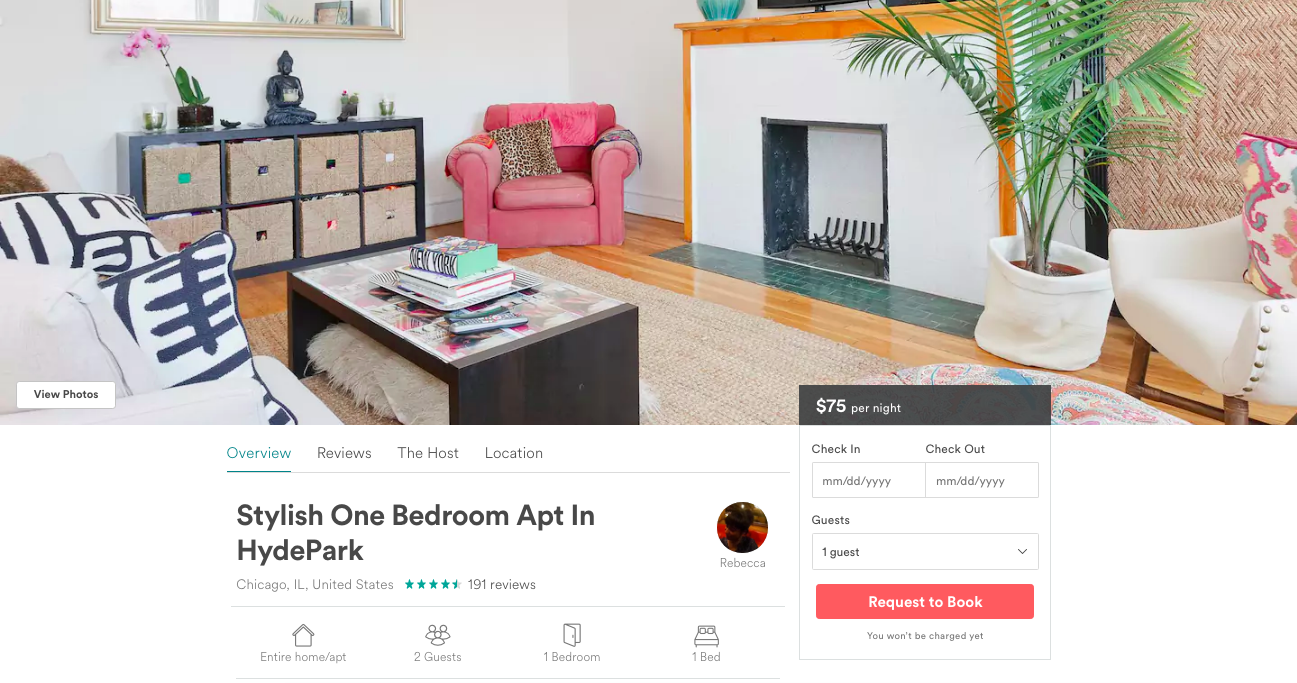
\includegraphics[width=1\textwidth]{tables/sample1-cover}
	\caption{Sample listing profile from Chicago}
	\label{fig:listing}
\end{figure}
\begin{figure}
%	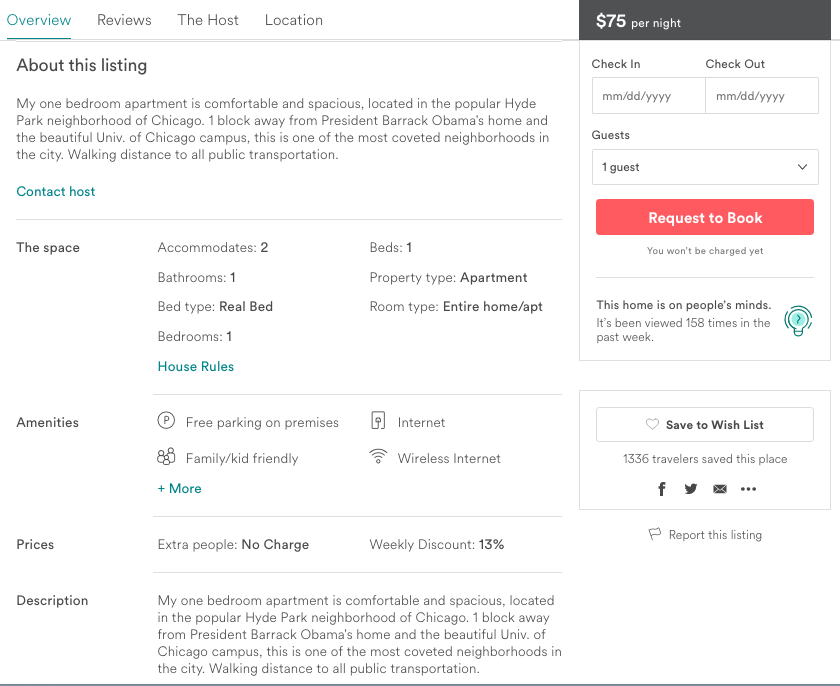
\includegraphics[width=1\textwidth]{tables/sample2-property}
	\caption{Sample property characteristics}
	\label{fig:property}
\end{figure}

%Histograms
\begin{figure}\centering
%	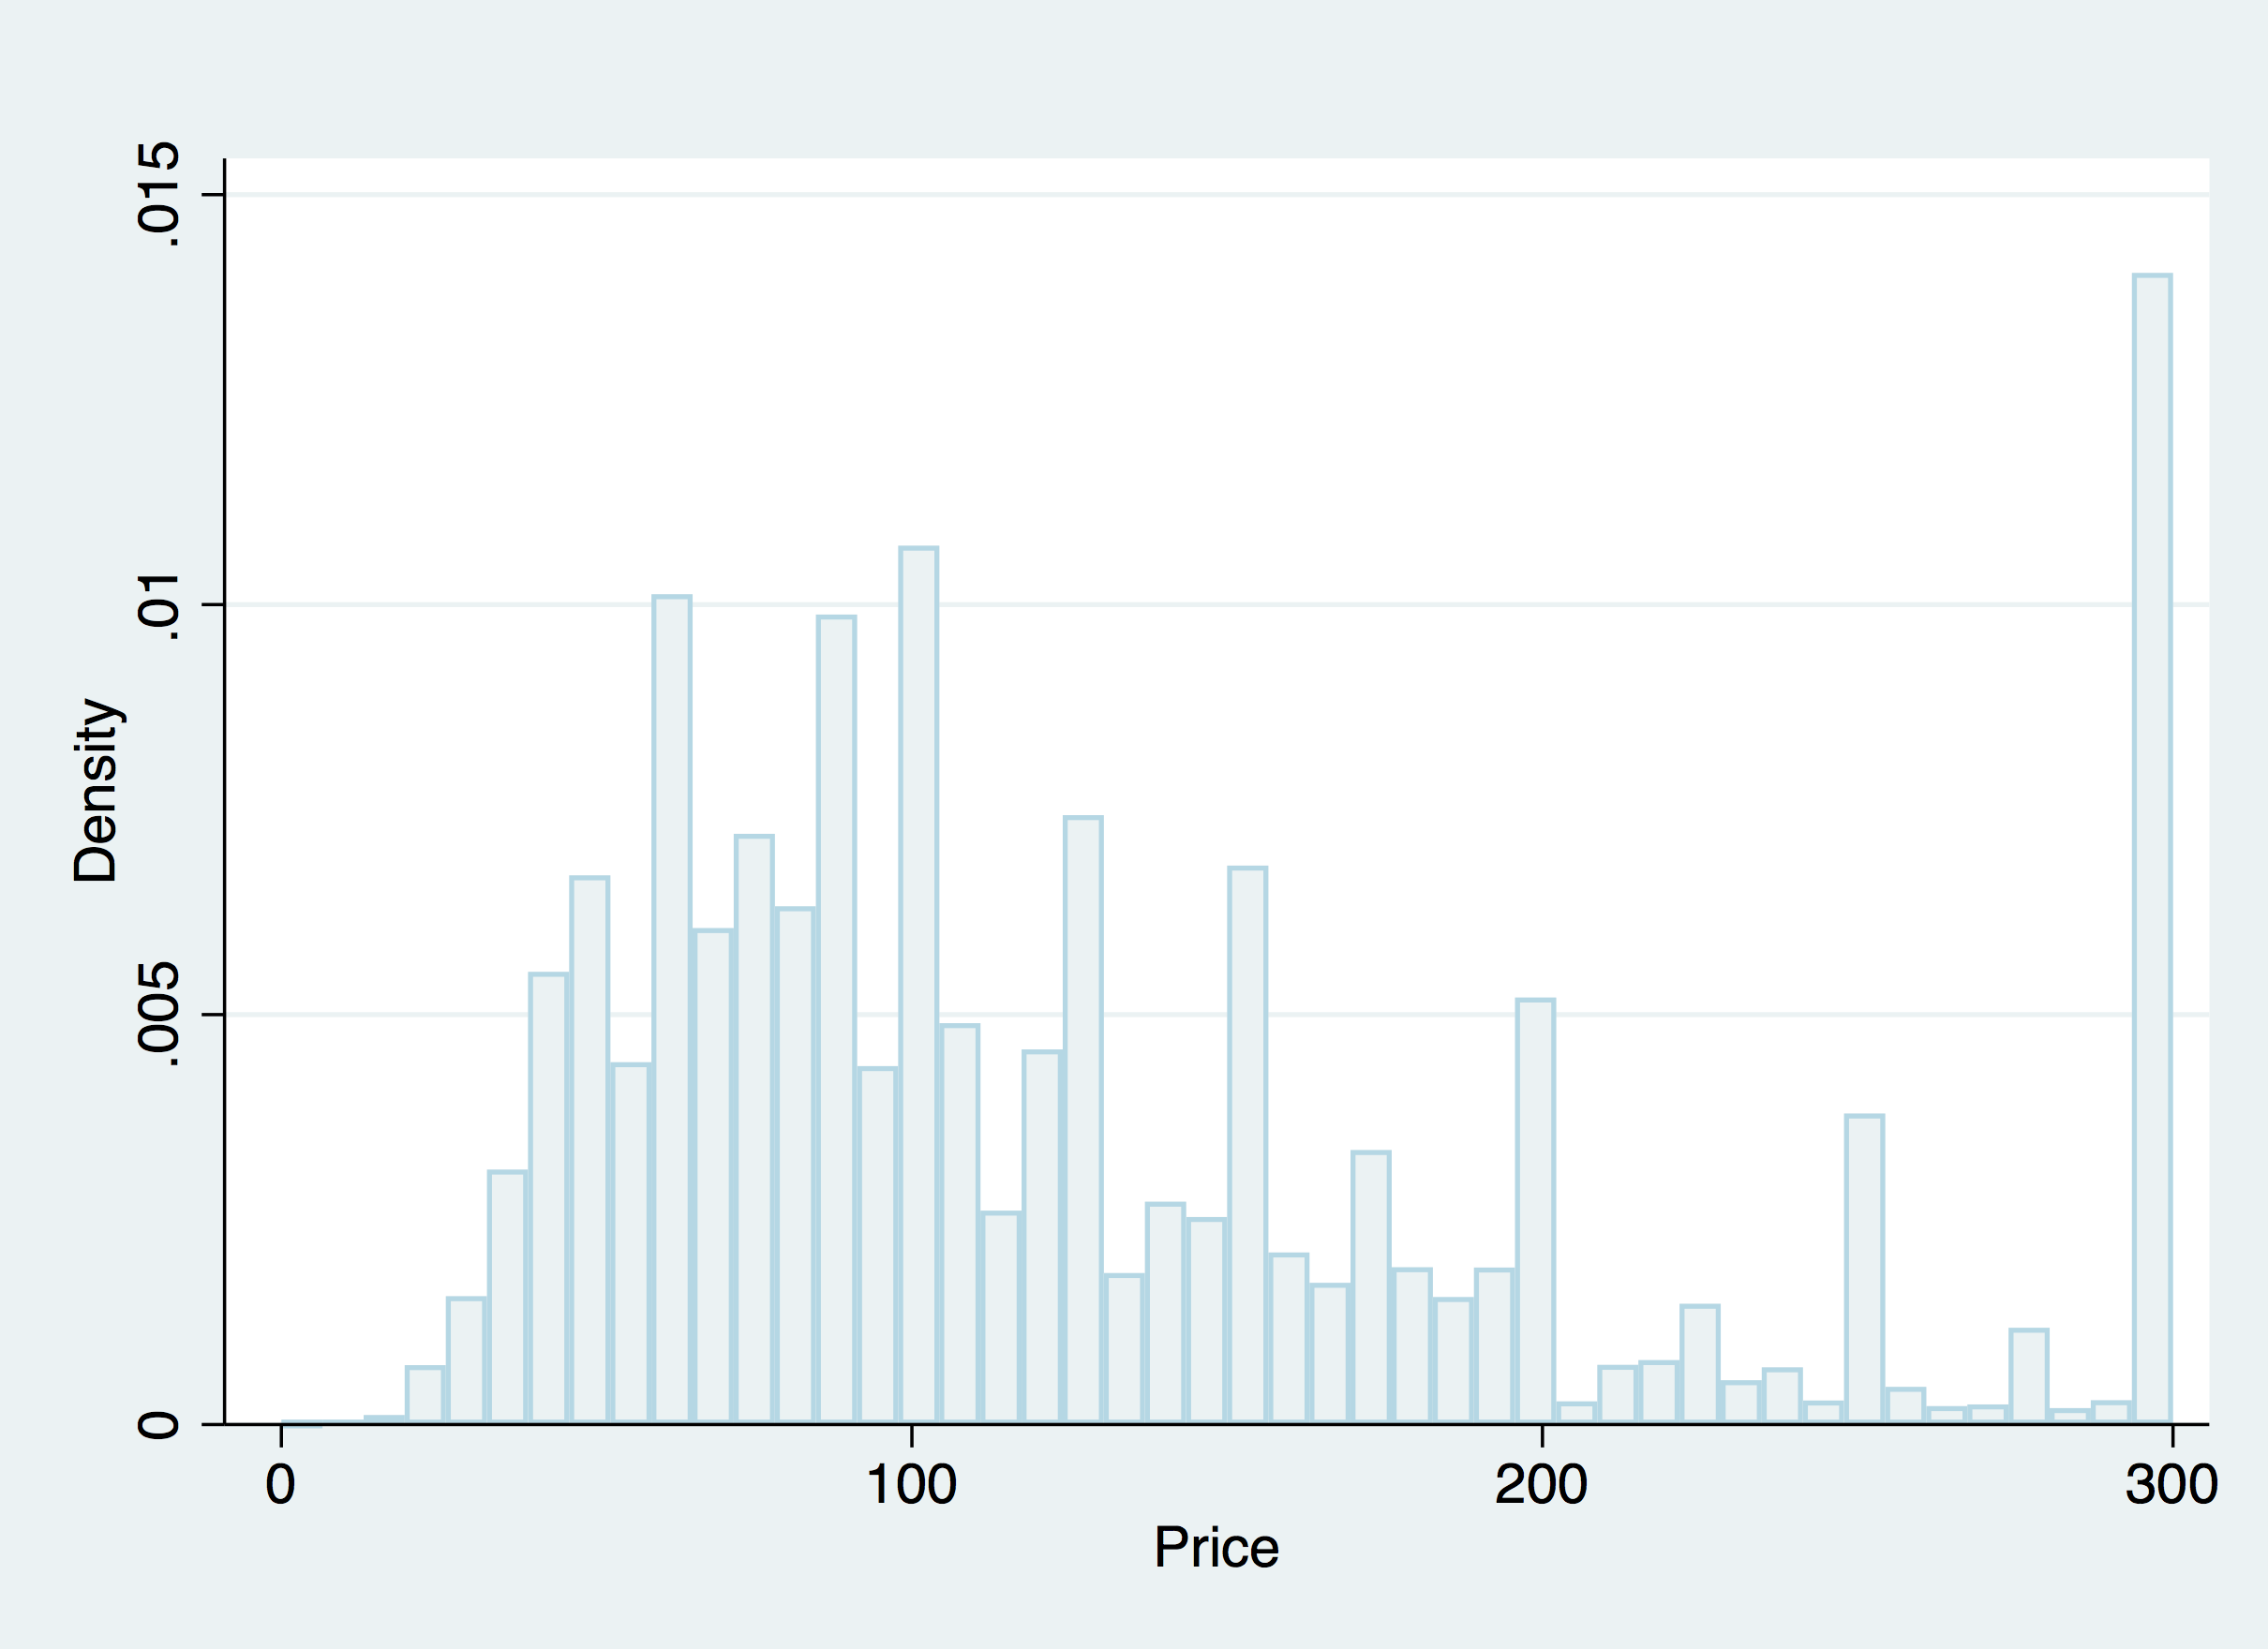
\includegraphics[width=.8\textwidth]{figures/price_dist-CONT-300}
	\caption{Distribution of prices}
	\caption*{Notes: All the listings priced at \$300 or more are grouped together at price = 300}
	\label{fig:prices}
\end{figure}

\begin{figure}\centering
%	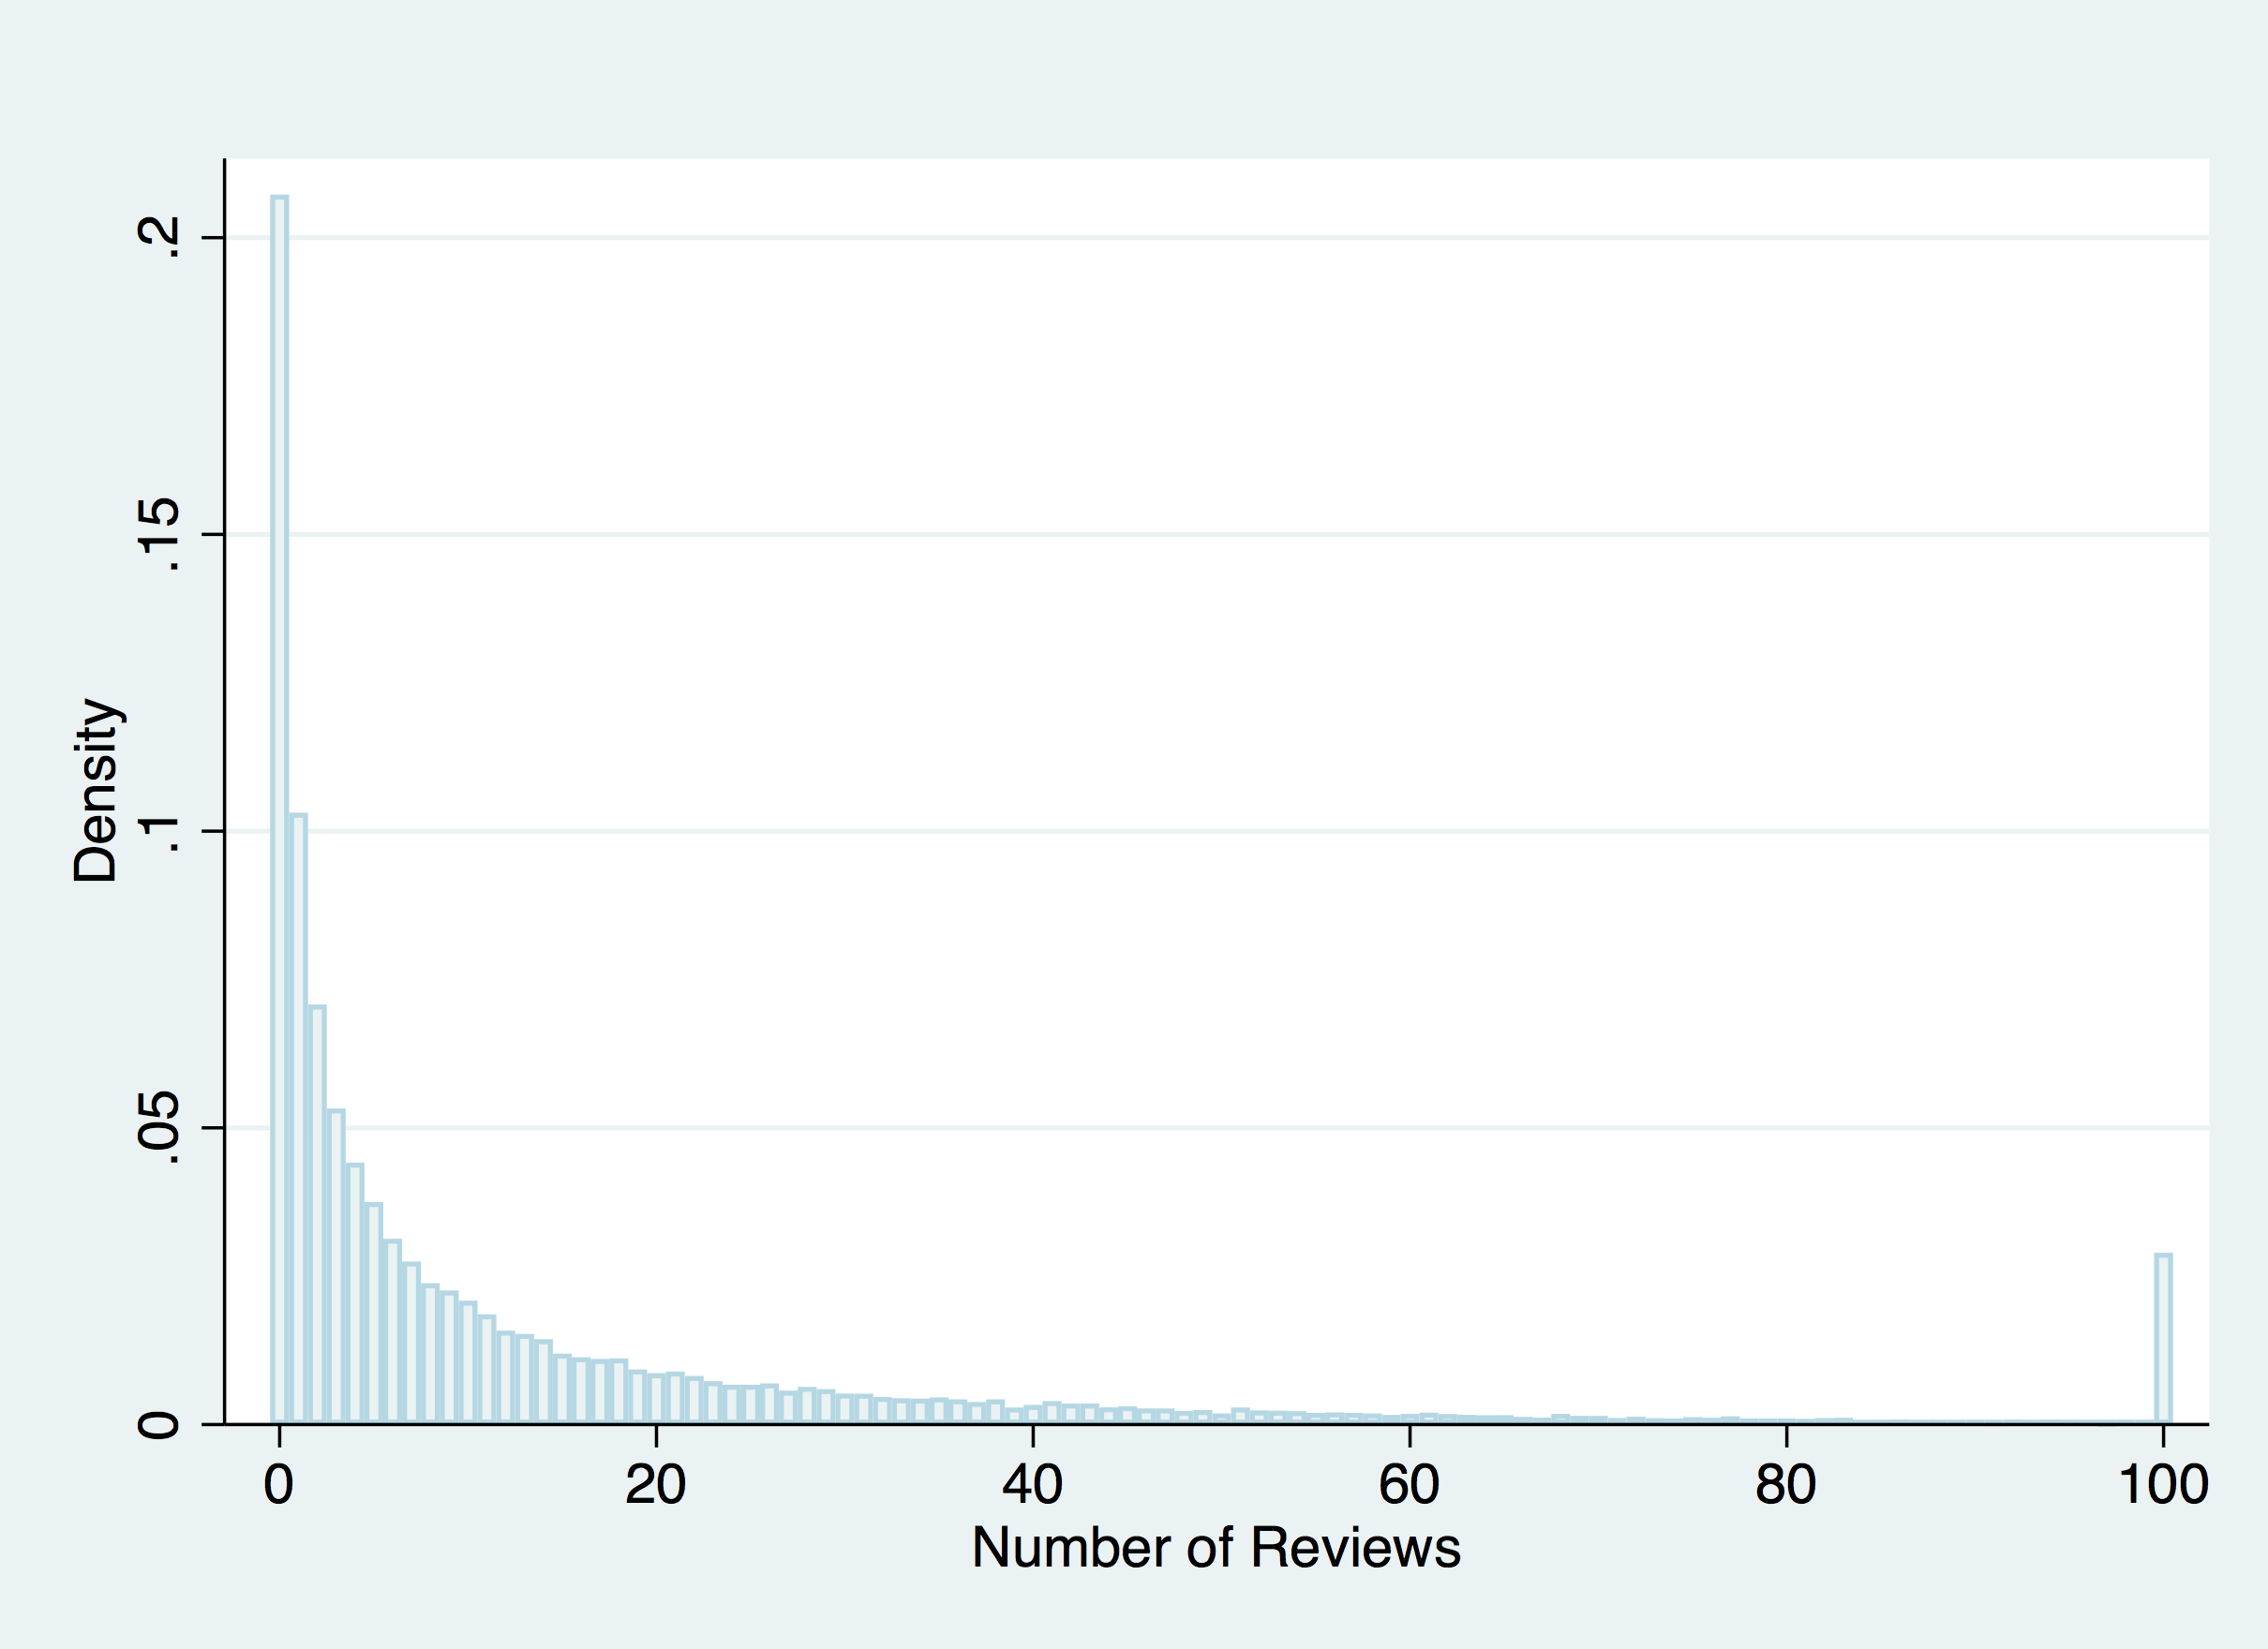
\includegraphics[width=.8\textwidth]{figures/num_reviews_dist-DISC-100}
	\caption{Distribution of number of reviews}
	\caption*{Notes: All the listings with 100 reviews or more are grouped together at number of reviews = 100}
	\label{fig:reviews}
\end{figure}

\begin{figure}\centering
%	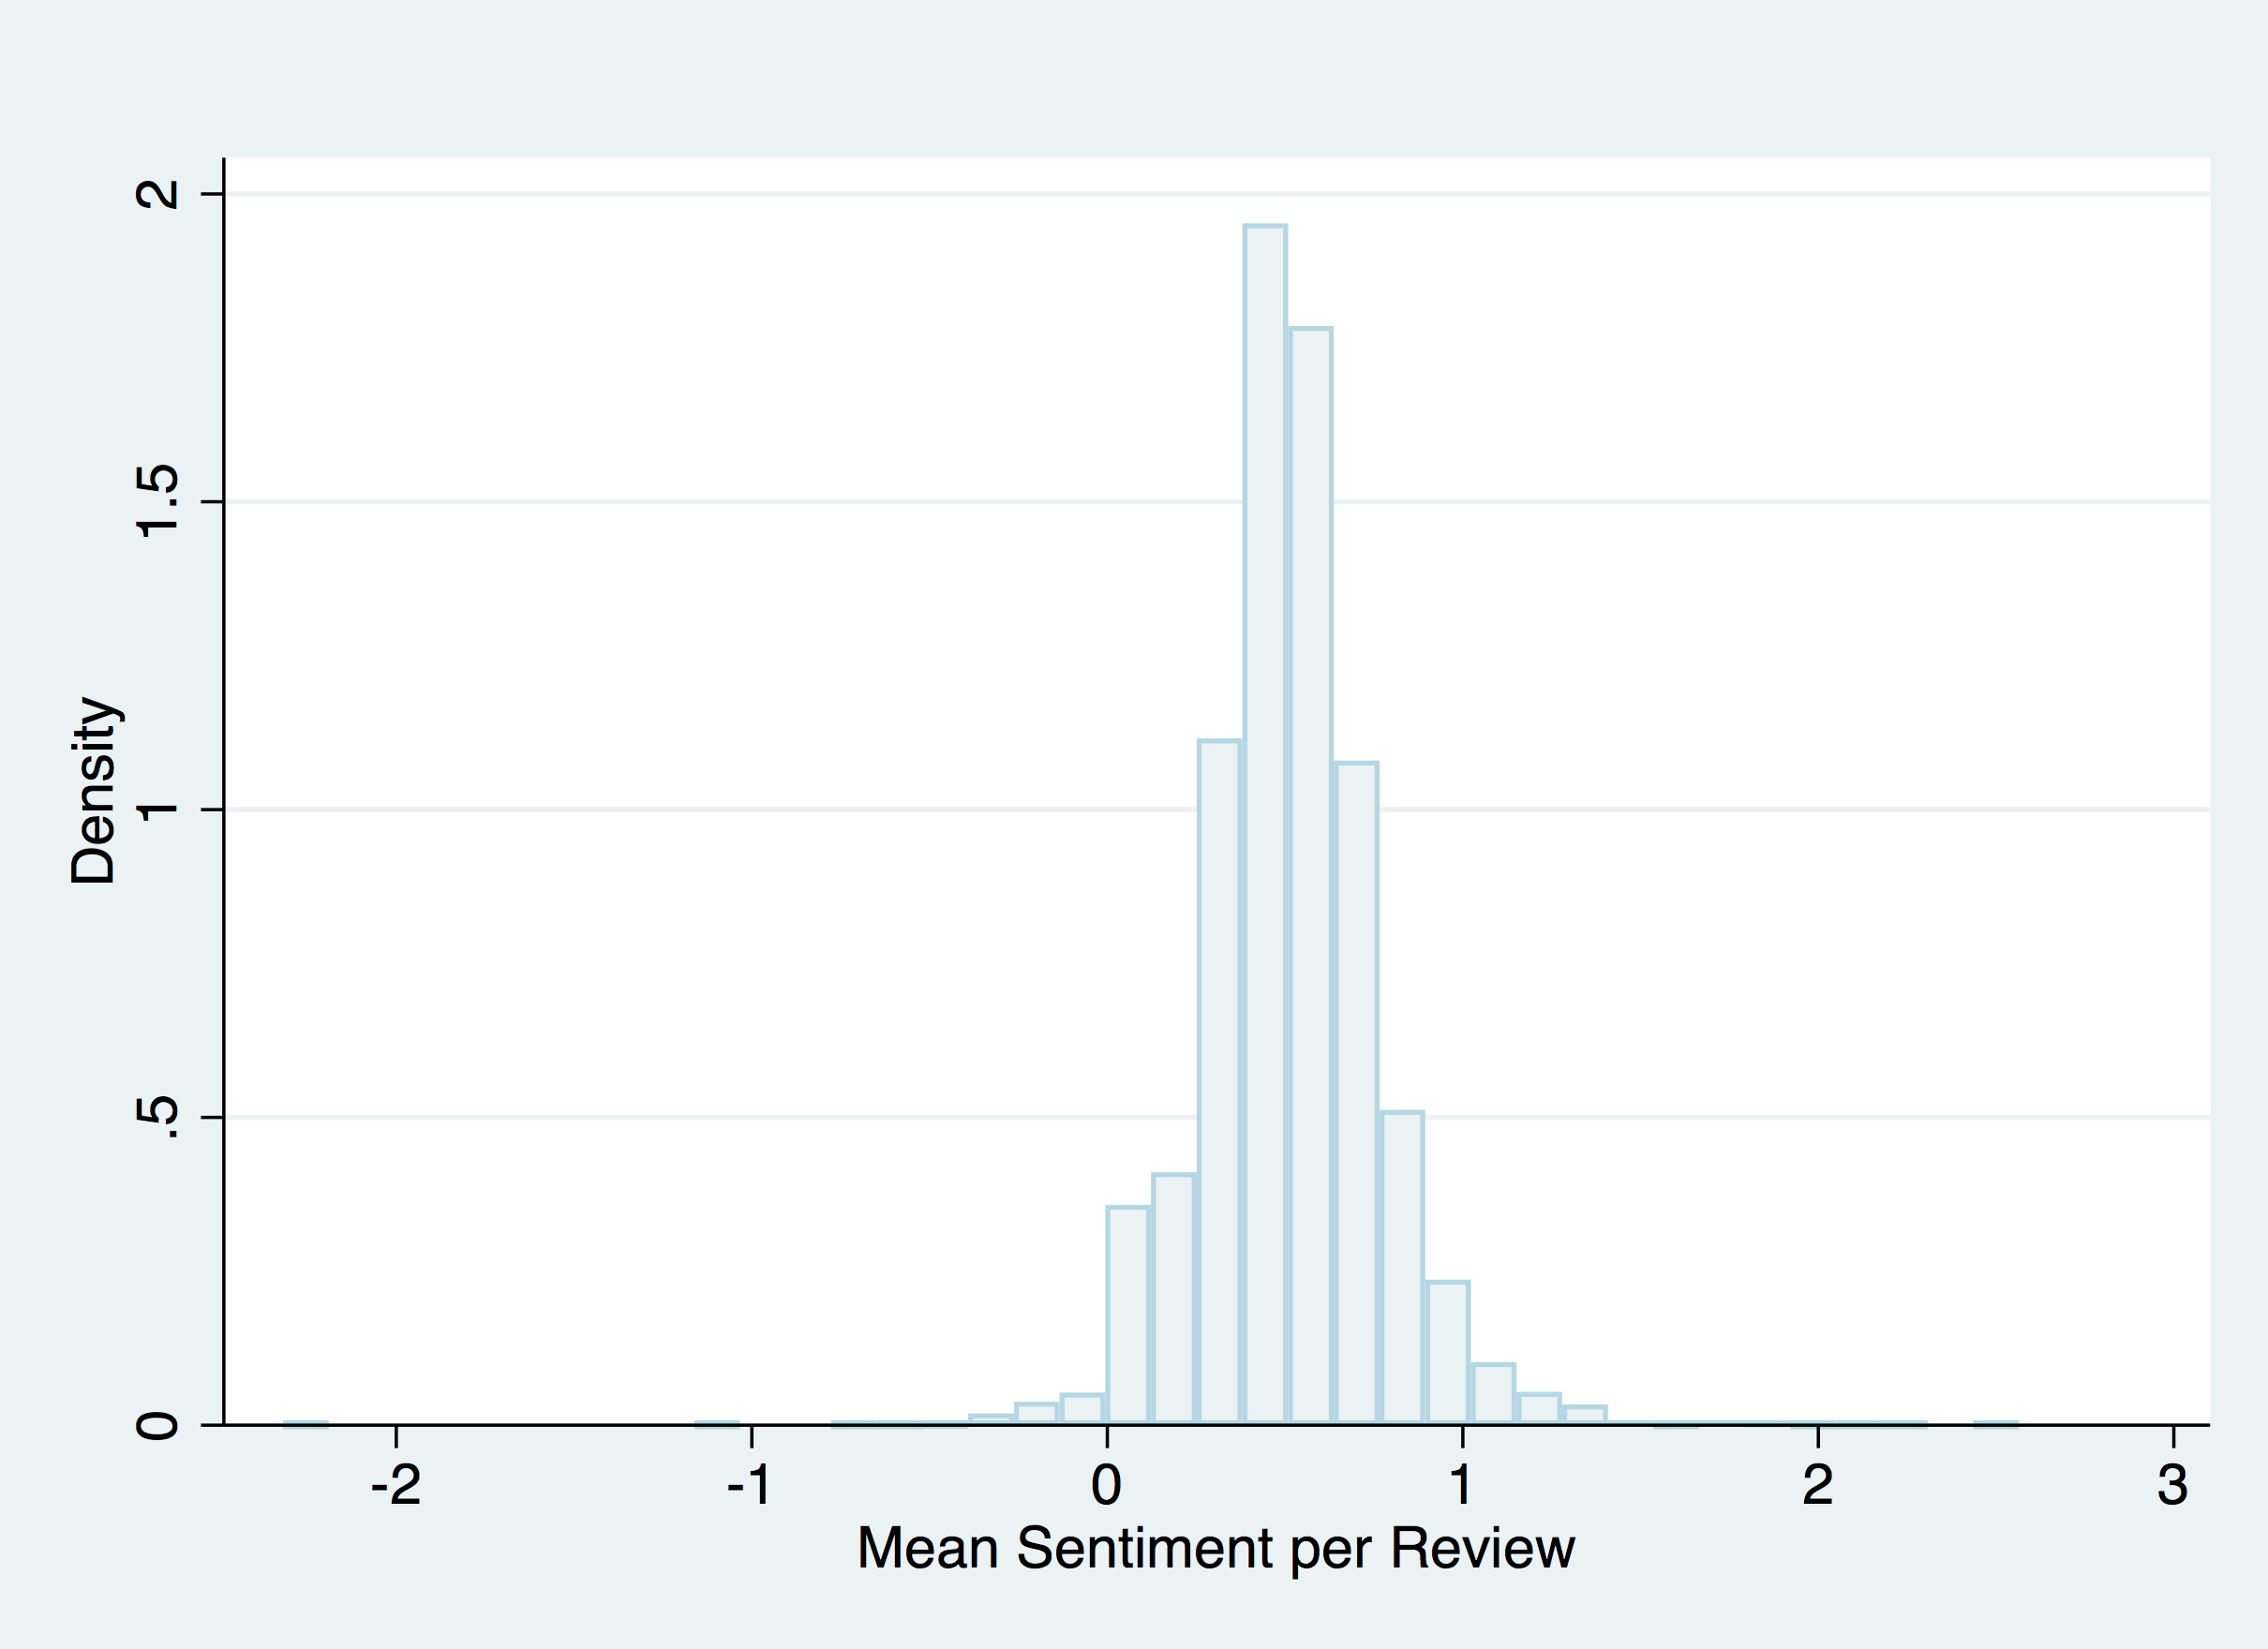
\includegraphics[width=.8\textwidth]{figures/review_sentiment_dist}
	\caption{Distribution of review sentiment}
	\label{fig:sentiment}
\end{figure}


%1
%listing-level summary table
\small
{
\begin{longtable}{l*{6}{c|c|cccc}}
	\caption{Summary Statistics by Host Race: Listing Characteristics}\\
	\hline
     &\multicolumn{1}{c}{Full data}&\multicolumn{1}{c}{}&\multicolumn{1}{c}{}&\multicolumn{1}{c}{Regression sample}&\multicolumn{1}{c}{}&\multicolumn{1}{c}{}\\
      \cline{3-7}\\
     &\multicolumn{1}{c}{}&\multicolumn{1}{c}{All}&\multicolumn{1}{c}{White}&\multicolumn{1}{c}{Black}&\multicolumn{1}{c}{Hispanic}&\multicolumn{1}{c}{Asian}\\
     \hline\hline
             
\textit{Outcome variables} \\
Price (\$/day)        & 175.72  &     167.37         &      178.62      &     125.95      &     160.39       &   131.06\\
                  & (294.14) &         (277.7)         &         (289.4)         &         (208.1)         &         (275.0)     & (242.1)    \\
Number of reviews     & 17.51  &      16.57  &      17.14         &      15.06&      16.46 & 	14.08\\
                 & (31.86)  &     (30.8)         &     (31.9)         &     (27.2)         &     (29.7)        & (27.6) \\
                 
\textit{Covariates} \\
\hline
Property Type \\
\hspace{3mm} Apartments/Lofts     		&	.577 &      .598         &       .590         &      .654        &      .625 			& 	.601         \\
\hspace{3mm} Townhouses/Condos   &  .042 &      .042         &      .039         &      .041        &      .041 	& 		.055         \\
\hspace{3mm} Houses    				&.321	&      .321         &       .336        &      .279        &      .289				& 		.311         \\
\hspace{3mm} Other    				&.06	&      .039      &       .035        &      .026        &      .045	& 		.033        \\

Room Type \\
\hspace{3mm} Entire home/apt   &  .577 & .577   	&      .607	&      .449  &      .510		&    .418\\
\hspace{3mm} Private room       & .384 & 	.384		&      .363	&      .483  &      .434		&    .530\\
\hspace{3mm} Shared room      & .039 &	.04	 	&      .029	&      .067  &      .056		&    .052\\

Max Num. Guests   & 3.44   &      3.26	&      3.36  &      2.90		&    3.17 		&	 2.89\\
               & (2.41)    &     (2.3)         &     (2.3)         &     (2.1)         &     (2.4)         & (2.1)\\
Bedrooms    &  1.35 &      1.30 &      1.33         &      1.20         &      1.25   & 1.20      \\
              &   (.92)   &     (.88)         &     (.92)         &     (.72)         &     (.90)       & (.76)  \\
Bathrooms  & 1.30  &      1.27         &       1.29         &      1.20         &      1.26 & 1.21         \\
                &  (.69)  &     (.66)         &     (.68)         &     (.52)         &     (.69)         & (.58)\\
Beds       & 1.82  &      1.73 &      1.76         &      1.63         &      1.74         & 1.59\\
               &   (1.41)  &     (1.32)         &     (1.31)         &     (1.22)         &     (1.60)   & (1.21)      \\
Availability (out of 30 days)    & 11.53   &      11.30&      10.9&      14.4 &      11.46  	& 	10.88\\
         &  (10.93)    & (10.99)     &     (10.85)  &     (11.54)  &     (11.03)         &     (11.05)         \\
Number of Amenities   &   .81  &      .80		&      .81&      .77 &      .80  	& 	.75\\
         						  &  (1.10)  & (1.10)     &     (1.11)    &     (1.05)         &     (1.10)         &     (1.13)         \\
Cleaning Fee   &  67.94 &      FIX	&      .81&      .77 &      .80  	& 	.75\\
						&  (60.36)  & (FIX)     &     (1.11)         &     (1.05)         &     (1.10)     &     (1.13)         \\
Extra Guests Charge   &   13.74  &  FIX      &    .81  &      .77           &   .80  	& 	.75\\
									&  (23.65)  & (1.10)  &     (1.11) &     (1.05)     &     (1.10) &     (1.13)  \\
Instantly Bookable?   &   .15  &      FIX		&      .81&      .77 &      .80  	& 	.75\\
									&  (.361)  & (1.10)     &     (1.11)  &     (1.05)   &     (1.10)   &     (1.13)         \\
Minimum Nights   &   3.01  &      FIX		&      .81&      .77 &      .80  	& 	.75\\
							&  (9.21)  & (1.10)     &     (1.11)         &     (1.05)         &     (1.10)         &     (1.13)         \\
Strict Cancellation Policy   &   .43  &      FIX		&      .81&      .77 &      .80  	& 	.75\\
[1em]
Year of first review    & 14.86   &      FIX	&      3.36  &      2.90		&    3.17 		&	 2.89\\
							& (1.22)    &     (FIX)         &     (2.3)         &     (2.1)         &     (2.4)         & (2.1)\\

\hline
Observations  & 69,007  & 68,983   &       43,988         &       5,023         &       3,524   & 5,893      \\
\hline\hline
\caption*{Notes: The values in the table are means and standard deviations of listing-level data in my full sample. Summary statistics for selected covariates are listed in the table. Categorical variables such as room type do not have standard deviations. Property types are explicitly listed if more than 1.5\% of listings are that type. Only the most popular cancellation policy type is listed - in the full sample, 99\% of listings have strict (43\%), flexible (31\%) or moderate (25\%) cancellation policies. Year of first review is a proxy for the time on the market - 14.86 indicates that the first review of the mean listing in the full sample occured in October of 2014.}

\end{longtable}
}
\normalsize




% \include{code/output/ }

%2
%Host-level summary table
{
	\def\sym#1{\ifmmode^{#1}\else\(^{#1}\)\fi}
	\begin{longtable}{l*{6}{c}}
		\caption{Summary Statistics by Race: Host Demographics}\\
		
		\hline
		&\multicolumn{1}{c}{}&\multicolumn{1}{c}{}&\multicolumn{1}{c}{}&\multicolumn{1}{c}{Regression}&\multicolumn{1}{c}{}&\multicolumn{1}{c}{}\\
		\cline{3-7}\\
			&\multicolumn{1}{c}{Full data}&\multicolumn{1}{c}{Full Sample}&\multicolumn{1}{c}{White}&\multicolumn{1}{c}{Black}&\multicolumn{1}{c}{Hispanic}&\multicolumn{1}{c}{Asian}\\
		
		\hline\hline\endfirsthead\hline\endhead\hline\endfoot\endlastfoot
		&\multicolumn{1}{c}{(1)}&\multicolumn{1}{c}{(2)}&\multicolumn{1}{c}{(3)}&\multicolumn{1}{c}{(4)}&\multicolumn{1}{c}{(5)}&\multicolumn{1}{c}{(6)}\\
		&\multicolumn{1}{c}{Full data}&\multicolumn{1}{c}{Regression sample}&\multicolumn{1}{c}{White}&\multicolumn{1}{c}{Black}&\multicolumn{1}{c}{Hispanic}&\multicolumn{1}{c}{Asian}\\
		\hline
		\endhead             
		     
		\textit{Host demographics} \\
		\hline
		\textit{Race} \\
		White     & &      .637         &       1.00         &      0         &      0 	& 		0         \\
		Black     &  &    .073       &       0         &      1.00         &      0 	& 		0         \\
		Hispanic     & &      .051         &       0         &      0         &      1.00 	& 		0         \\
		Asian     &   &   .085      &       0         &      0         &      0 	& 		1.00         \\
		Unknown/Multiracial     & &      .152         &       0         &      0         &      0 	& 		0         \\
		[1em]
		\textit{Sex} \\
		Male     & &      .309         &       .356         &      .354         &      .417 	& 		.367        \\
		Female     & &      .378         &       .427        &      .541         &      .426 	& 		.476         \\
		Unknown/Two people   &  &      .312         &       .216         &      .104         &      .156 	& 		.157         \\
		[1em]
		\textit{Age} \\
		Young ($<$ 30)     & &      .427         &       .469         &      .514        &      .481 	& 		.587         \\
		Middle-aged     & &      .421         &       .491        &      .470         &      .490 		& 		.379         \\
		Old ($>$ 65)     & &      .018         &       .026         &      .004         &      .009	& 		.009         \\
		Unknown    &  &      .133         &       .013         &      .011         &      .018 	& 		.024         \\
		[1em]

		
		\hline
		Observations (full sample)    &  & 68,983   &       43,988         &       5,023         &       3,524         &       5,893         \\
		\hline\hline
		\caption*{Notes: The values in the table are means and standard deviations of host-level data in my full sample. Summary statistics for selected covariates are listed in the table. Categorical variables such as race, sex, and age do not have standard deviations. White refers only to Non-Hispanic Whites.}
		
	\end{longtable}
}



%3
%Host-level summary table
{
	\def\sym#1{\ifmmode^{#1}\else\(^{#1}\)\fi}
	\begin{longtable}{l*{6}{c}}
		\caption{Summary Statistics by Race: Host Characteristics}\\
		
		\hline
		&\multicolumn{1}{c}{}&\multicolumn{1}{c}{}&\multicolumn{1}{c}{}&\multicolumn{1}{c}{Regression}&\multicolumn{1}{c}{}&\multicolumn{1}{c}{}\\
		\cline{3-7}\\
			&\multicolumn{1}{c}{Full data}&\multicolumn{1}{c}{Full Sample}&\multicolumn{1}{c}{White}&\multicolumn{1}{c}{Black}&\multicolumn{1}{c}{Hispanic}&\multicolumn{1}{c}{Asian}\\
		
		\hline\hline\endfirsthead\hline\endhead\hline\endfoot\endlastfoot
		&\multicolumn{1}{c}{(1)}&\multicolumn{1}{c}{(2)}&\multicolumn{1}{c}{(3)}&\multicolumn{1}{c}{(4)}&\multicolumn{1}{c}{(5)}&\multicolumn{1}{c}{(6)}\\
		&\multicolumn{1}{c}{Full data}&\multicolumn{1}{c}{Regression sample}&\multicolumn{1}{c}{White}&\multicolumn{1}{c}{Black}&\multicolumn{1}{c}{Hispanic}&\multicolumn{1}{c}{Asian}\\
		\hline
		\endhead             
		     
		\textit{Outcome variables} \\
		Host listings count         & &      5.53&      5.50 &      10.5&    3.16 & 2.68\\
		&	&     (33.0)         &     (31.2)         &     (60.3)         &     (17.8) & 	(3.62)         \\
		[1em]
		\textit{Selected covariates} \\
		\hline\hline
		\textit{Host characteristics} \\
		\hline
		Review value      &   &      93.61	&      94.08	 	&      91.89		&    92.81	 & 		92.24\\
		(out of 100)              &      &     (8.00)         &     (7.49)         &     (9.42)         &     (8.72) 	&	 (9.27)         \\
		[1em]
		Host is a superhost    &    &      .124		&      .134&      .084 &      .108  	& 	.097\\
		& & (.329)     &     (.341)         &     (.277)         &     (.310)         &     (.296)         \\
		[1em]
		Response rate      &   &       .756		&       .756		&      .771         &      .756  	& 	.744\\
		& &     (.391)         &     (.393)         &     (.368)         &     (.386)         &		(.399)\\
		[1em]
		Acceptance rate      &     &      .453&      .463&       .357         &      .494    &	.446     \\
		& &     (.463)         &     (.463)         &     (.451)         &     (.466)         &		(.467)\\
		[1em]
		Total ``good" words       &    &      .655&      .656&       .686         &      .677    &	.604     \\
		& &     (.857)         &     (.843)         &     (.882)         &     (.867)         &		(.826)\\
		[1em]
		Length of ``Summary"      &     &      208.67 	&      210.20	&       203.25         &      206.74    &	205.81     \\
		& &       (64.99)  &    (64.08)         &     (70.59)         &     (65.62)         &     (65.87) \\
		[1em]
		Short words in ``Summary"          &  &      .182		&      .185		&       .187         &      .175    &	.175     \\
		& &     (1.19)         &     (1.15)         &     (1.24)         &     (1.26)         &		(1.32)\\                    
		
		
		\hline
		Observations (full sample)    &  & 68,983   &       43,988         &       5,023         &       3,524         &       5,893         \\
		\hline\hline
		\caption*{Notes: The values in the table are means and standard deviations of host-level data in my full sample. Summary statistics for selected covariates are listed in the table. Categorical variables such as race, sex, and age do not have standard deviations. White refers only to Non-Hispanic Whites. Length of ``Summary" and proportion of short words in the ``Summary'' refer to my constructed measures of host quality. These two measures were also calculated for the description, space, neighborhood overview, notes, and transit fields, but were not included in the table for the sake of clarity and because they follow a similar pattern as the ``Summary" field.}
		
	\end{longtable}
}



%4
% reviewer summary table

{
	\def\sym#1{\ifmmode^{#1}\else\(^{#1}\)\fi}
	\begin{longtable}{l*{5}{c}}
		\caption{Summary Statistics by Race: Reviewer Characteristics}\\
		\hline
		&\multicolumn{1}{c}{(1)}&\multicolumn{1}{c}{(2)}&\multicolumn{1}{c}{(3)}&\multicolumn{1}{c}{(4)}&\multicolumn{1}{c}{(5)}\\
		&\multicolumn{1}{c}{Full sample}&\multicolumn{1}{c}{White}&\multicolumn{1}{c}{Black}&\multicolumn{1}{c}{Hispanic}&\multicolumn{1}{c}{Asian}\\
		\hline\hline\endfirsthead\hline\endhead\hline\endfoot\endlastfoot
		&\multicolumn{1}{c}{(1)}&\multicolumn{1}{c}{(2)}&\multicolumn{1}{c}{(3)}&\multicolumn{1}{c}{(4)}&\multicolumn{1}{c}{(5)}\\
		&\multicolumn{1}{c}{Full sample}&\multicolumn{1}{c}{White}&\multicolumn{1}{c}{Black}&\multicolumn{1}{c}{Hispanic}&\multicolumn{1}{c}{Asian}\\
		\hline
		\endhead                  

		\textit{Reviewer characteristics (Chicago data only) } \\
		\hline
		Host race            &      1.00 &      .738&       .099         &      .079    &	.083     \\
		[1em]
		Reviewer race            &      1.00		&      .759	&       .041         &      .047    &	.153     \\
		[1em]
		Review sentiment            &      .510	&      .512&       .503         &      .509    &	.506     \\
		&     (.261)         &     (.254)         &     (.258)         &     (.276)         &		(.287)\\
		[1em]
		Listing sentiment            &      .507&      .509&       .502         &      .499    &	.506     \\
		&     (.072)         &     (.067)         &     (.089)         &     (.096)         &		(.094)\\
		
		\hline
		Observations (full sample)     & 68,983   &       43,988         &       5,023         &       3,524         &       5,893         \\
		\hline\hline
		\caption*{Notes: The values in the table are means and standard deviations of reviewer-level data of a randomly chosen set of hosts in Chicago. Categorical variables do not have standard deviations. White refers only to Non-Hispanic Whites. The host race and the reviewer race in that panel is the proportion of each race that are included in the Reviewer data. The review sentiment is the sentiment of each review, the listing sentiment is the average sentiment per listing.}
		
	\end{longtable}
}



%5 - Main
{
\def\sym#1{\ifmmode^{#1}\else\(^{#1}\)\fi}
\begin{longtable}{l*{4}{c}}
\caption{Main result: Estimates of effect of host's race and gender on price}\\
\hline\hline\endfirsthead\hline\endhead\hline\endfoot\endlastfoot
                    &\multicolumn{1}{c}{(1)}&\multicolumn{1}{c}{(2)}&\multicolumn{1}{c}{(3)}&\multicolumn{1}{c}{(4)}\\
                    &\multicolumn{1}{c}{Price}&\multicolumn{1}{c}{Price}&\multicolumn{1}{c}{Price}&\multicolumn{1}{c}{Price}\\
\hline
White Female        &      -3.727\sym{*}  &      -3.714\sym{*}  &      -0.827         &      -0.243         \\
                    &     (1.770)         &     (1.562)         &     (1.049)         &     (1.053)         \\
[1em]
Black Male          &      -39.43\sym{***}&      -14.24\sym{***}&      -6.891\sym{***}&      -6.917\sym{***}\\
                    &     (4.058)         &     (3.483)         &     (1.994)         &     (1.963)         \\
[1em]
Black Female        &      -41.69\sym{***}&      -11.20\sym{***}&      -6.271\sym{***}&      -5.793\sym{***}\\
                    &     (4.315)         &     (2.793)         &     (1.577)         &     (1.586)         \\
[1em]
Hispanic Male       &      -20.59\sym{***}&      -7.247\sym{**} &      -2.537         &      -2.165         \\
                    &     (3.727)         &     (2.759)         &     (2.051)         &     (2.073)         \\
[1em]
Hispanic Female     &      -23.05\sym{***}&      -11.38\sym{***}&      -5.284\sym{*}  &      -5.022\sym{*}  \\
                    &     (4.426)         &     (3.219)         &     (2.110)         &     (2.078)         \\
[1em]
Asian Male          &      -27.42\sym{***}&      -12.08\sym{***}&      -5.834\sym{**} &      -6.338\sym{**} \\
                    &     (4.954)         &     (3.553)         &     (2.206)         &     (2.185)         \\
[1em]
Asian Female        &      -39.18\sym{***}&      -21.20\sym{***}&      -8.611\sym{***}&      -8.604\sym{***}\\
                    &     (4.463)         &     (2.592)         &     (1.586)         &     (1.599)         \\
[1em]
Constant            &       147.4\sym{***}&       54.75\sym{***}&      -33.93\sym{***}&      -0.742         \\
                    &     (5.015)         &     (1.506)         &     (5.507)         &     (6.764)         \\
\hline
Controls:        \\
\hspace{3mm} Location  &                &       X         &       X         &       X         \\
\hspace{3mm} Property Characteristics  &                &                &       X         &       X         \\
\hspace{3mm} Host Characteristics  &                &                &                &       X         \\
\hline
Observations        &       45072         &       45072         &       45072         &       45072         \\
Adjusted \(R^{2}\)  &       0.019         &       0.166         &       0.621         &       0.627         \\
\hline\hline
\multicolumn{5}{l}{\footnotesize Standard errors in parentheses}\\
\multicolumn{5}{l}{\footnotesize \sym{*} \(p<0.05\), \sym{**} \(p<0.01\), \sym{***} \(p<0.001\)}\\
\caption*{Notes: The dependent variable is the price of the listing. All race coefficients are relative to white males. The unit of observation is a listing. The sample is the sample of listings across 7 US cities. Model 1 is the baseline effect of host demographics on price. Model 2 controls for listing location to the neighborhood level. Model 3 adds listing characteristics such as property type, time on market, number of bedrooms, availability, etc. Model 4 adds host characteristics such as response and acceptance rates, measures of host effort, Superhost status, etc. See Data Appendix for full description of covariates.}
\label{Table 4}


\end{longtable}
}


\begin{comment}
[1em]
Middle-aged         &       12.21\sym{***}&       10.62\sym{***}&       1.724         &       1.702         \\
&     (2.126)         &     (1.281)         &     (0.913)         &     (0.907)         \\
[1em]
Old ($>$ 65)           &       8.145         &       3.664         &      -1.752         &      -2.239         \\
&     (5.936)         &     (5.339)         &     (3.271)         &     (3.237)         \\
	
\end{comment}


\begin{table}[htbp]\centering
	\def\sym#1{\ifmmode^{#1}\else\(^{#1}\)\fi}
	\caption{New title here}
	\label{table:price_new}
	\begin{tabular}{c|ccccc}
		\toprule
		
		                    &\multicolumn{1}{c}{(1)}&\multicolumn{1}{c}{(2)}&\multicolumn{1}{c}{(3)}&\multicolumn{1}{c}{(4)}&\multicolumn{1}{c}{(5)}\\
                    &\multicolumn{1}{c}{Model 1}&\multicolumn{1}{c}{Model 2}&\multicolumn{1}{c}{Model 3}&\multicolumn{1}{c}{Model 4}&\multicolumn{1}{c}{Model 5}\\
\hline
White Male          &       31.25         &      -27.80         &       103.8         &       92.84         &       95.59         \\
                    &     (147.6)         &     (113.8)         &     (104.7)         &     (102.0)         &     (104.8)         \\
[1em]
White Female        &       26.23         &      -34.57         &       105.2         &       95.84         &       98.69         \\
                    &     (148.4)         &     (114.2)         &     (105.3)         &     (102.7)         &     (105.6)         \\
[1em]
Black Male          &      -28.02         &      -48.15         &       95.73         &       83.76         &       85.77         \\
                    &     (146.3)         &     (115.5)         &     (106.0)         &     (103.1)         &     (106.0)         \\
[1em]
Black Female        &      -19.77         &      -36.85         &       102.6         &       92.59         &       95.22         \\
                    &     (144.9)         &     (113.3)         &     (104.8)         &     (102.2)         &     (105.1)         \\
[1em]
Hispanic Male       &       9.268         &      -31.14         &       110.2         &       99.87         &       102.6         \\
                    &     (146.6)         &     (114.6)         &     (105.5)         &     (102.8)         &     (105.6)         \\
[1em]
Hispanic Female     &       12.35         &      -36.73         &       100.8         &       90.28         &       91.93         \\
                    &     (146.0)         &     (113.9)         &     (105.6)         &     (102.9)         &     (105.6)         \\
[1em]
Asian Male          &      -10.64         &      -48.36         &       92.58         &       80.60         &       82.58         \\
                    &     (144.5)         &     (113.1)         &     (104.3)         &     (101.6)         &     (104.4)         \\
[1em]
Asian Female        &      -20.84         &      -53.02         &       100.9         &       90.40         &       92.43         \\
                    &     (144.6)         &     (114.0)         &     (105.5)         &     (102.9)         &     (105.7)         \\
\hline
Location Fixed Effects&                     &         Yes         &         Yes         &         Yes         &         Yes         \\
Property Fixed Effects&                     &                     &         Yes         &         Yes         &         Yes         \\
Host Fixed Effects  &                     &                     &                     &         Yes         &         Yes         \\
\hline \vspace{-1.25em}&                     &                     &                     &                     &                     \\
Observations        &       46926         &       46926         &       46926         &       46902         &       46902         \\
Adjusted R2         &     0.00700         &       0.119         &       0.387         &       0.390         &       0.390         \\

		
		\bottomrule
	\end{tabular}
	
	\begin{tablenotes}
		\item \footnotesize Standard errors in parentheses
		\item \footnotesize \sym{*} \(p<0.05\), \sym{**} \(p<0.01\), \sym{***} \(p<0.001\)
		
		\item Notes: The dependent variable is the price of the listing. All race coefficients are relative to white males. The unit of observation is a listing. The sample is the sample of listings across 7 US cities. Model 1 is the baseline effect of host demographics on price. Model 2 controls for listing location to the neighborhood level. Model 3 adds listing characteristics such as property type, time on market, number of bedrooms, availability, etc. Model 4 adds host characteristics such as response and acceptance rates, measures of host effort, Superhost status, etc. See Data Appendix for full description of covariates.  
	\end{tablenotes}
\end{table}



%6
{
\def\sym#1{\ifmmode^{#1}\else\(^{#1}\)\fi}
\begin{longtable}{l*{1}{c}}
\caption{Robustness check with controls from Edelman \& Luca (2014), NYC data}\\
\hline\hline\endfirsthead\hline\endhead\hline\endfoot\endlastfoot
                    &\multicolumn{1}{c}{(1)}\\
                    &\multicolumn{1}{c}{Price per night}\\
\hline
Black               &      -18.11\sym{***}\\
                    &     (1.813)         \\
Accommodates        &       12.84\sym{***}\\
                    &     (0.488)         \\
Bedrooms            &       33.60\sym{***}\\
                    &     (1.227)         \\
Review Scores Location&      -74.66\sym{***}\\
                    &     (7.363)         \\
Review Scores Location Squared           &       5.407\sym{***}\\
                    &     (0.421)         \\

Review Scores Checkin&      -1.268         \\
                    &     (1.157)         \\
Review Scores Communication&      -1.226         \\
                    &     (1.218)         \\
Review Scores Cleanliness&       3.454\sym{***}\\
                    &     (0.706)         \\
Review Scores Accuracy&      -1.479         \\
                    &     (0.973)         \\
Host verified &       1.945         \\
                    &     (1.357)         \\
Private room        &      -71.14\sym{***}\\
                    &     (1.400)         \\
Shared room         &      -102.8\sym{***}\\
                    &     (3.109)         \\
\hline
Controls:        \\
\hspace{3mm} Location  &                           X      \\
\hspace{3mm} Property Characteristics  &   X         \\
\hspace{3mm} Host Characteristics  &         X        \\
\hline
Observations        &       11999         \\
Adjusted \(R^{2}\)  &       0.526         \\
\hline\hline
\multicolumn{2}{l}{\footnotesize Standard errors in parentheses}\\
\multicolumn{2}{l}{\footnotesize \sym{*} \(p<0.05\), \sym{**} \(p<0.01\), \sym{***} \(p<0.001\)}\\
\caption*{\footnotesize Notes: This table presents the effect on price of controlling for Edelman \& Luca's (2014) full specification using my NYC data. The results are nearly identical to theirs (their coefficient on Black hosts was -17.8) when controlling for similar covariates in the same city. The omitted category for race is white hosts. The omitted category for room type is Entire Apartment. I could not control for host social media accounts as a proxy for host reliability like Edelman \& Luca, because Airbnb no longer provides this information. Instead, I controlled for ``host verified", a boolean for whether Airbnb has the host's phone number and email. I was not able to control for ``picture quality" either, but picture quality did not significantly influence price in Edelman \& Luca's regression.}\\
\end{longtable}
}




\begin{table}[htbp]\centering
	\def\sym#1{\ifmmode^{#1}\else\(^{#1}\)\fi}
	\caption{New title here}
	\label{table:edelman_new}
	\begin{tabular}{c|c}
		\toprule
		
		                    &\multicolumn{1}{c}{(1)}\\
                    &\multicolumn{1}{c}{Edelman}\\
\hline
0                   &           0         \\
                    &         (.)         \\
[1em]
White               &      -2.787         \\
                    &     (70.53)         \\
[1em]
Black               &      -21.11         \\
                    &     (70.60)         \\
[1em]
Hispanic            &      -15.34         \\
                    &     (70.70)         \\
[1em]
Asian               &      -3.804         \\
                    &     (70.61)         \\
\hline
Location Fixed Effects&         Yes         \\
Property Fixed Effects&         Yes         \\
Host Fixed Effects  &         Yes         \\
\hline \vspace{-1.25em}&                     \\
Observations        &       12129         \\
Adjusted R2         &       0.224         \\

		
		\bottomrule
	\end{tabular}
	
	\begin{tablenotes}
		\item \footnotesize Standard errors in parentheses
		\item \footnotesize \sym{*} \(p<0.05\), \sym{**} \(p<0.01\), \sym{***} \(p<0.001\)
		
		\item Notes: This table presents the effect on price of controlling for Edelman \& Luca's (2014) full specification using my NYC data. My results are nearly identical to theirs (their coefficient on Black *hosts was -17.8) when controlling for similar covariates in the same city. The omitted category for race is White hosts. The omitted category for room type is Entire Apartment. I could not control for host social media accounts as a proxy for host reliability like Edelman \& Luca did, because Airbnb no longer provides this information. Instead, I controlled for ``host verified", a boolean for whether Airbnb has the host's phone number and email. I was not able to control for ``picture quality" either, but picture quality did not significantly influence price in Edelman \& Luca's regression.
	\end{tablenotes}
\end{table}


%7
{
\def\sym#1{\ifmmode^{#1}\else\(^{#1}\)\fi}
\begin{longtable}{l*{4}{c}}
\caption{Estimates of effect of host's race and gender on number of reviews}\\
\hline\hline\endfirsthead\hline\endhead\hline\endfoot\endlastfoot
                    &\multicolumn{1}{c}{(1)}&\multicolumn{1}{c}{(2)}&\multicolumn{1}{c}{(3)}&\multicolumn{1}{c}{(4)}\\
\hline
White Female        &      -0.804         &      -0.560         &      -1.420\sym{***}&      -1.362\sym{***}\\
                    &     (0.540)         &     (0.496)         &     (0.344)         &     (0.338)         \\
[1em]
Black Male          &      -2.049         &      -1.494         &      -2.034\sym{**} &      -1.287\sym{*}  \\
                    &     (1.137)         &     (0.970)         &     (0.617)         &     (0.599)         \\
[1em]
Black Female        &      -2.153         &      -1.439         &      -2.523\sym{***}&      -2.330\sym{***}\\
                    &     (1.125)         &     (1.004)         &     (0.559)         &     (0.536)         \\
[1em]
Hispanic Male       &      -1.404         &      -0.168         &      -0.183         &    -0.00232         \\
                    &     (1.258)         &     (1.178)         &     (0.817)         &     (0.797)         \\
[1em]
Hispanic Female     &      -0.443         &       0.805         &      -0.867         &      -0.462         \\
                    &     (1.119)         &     (1.042)         &     (0.749)         &     (0.704)         \\
[1em]
Asian Male          &      -2.856\sym{**} &      -1.054         &      -1.024         &      -1.030         \\
                    &     (0.913)         &     (0.832)         &     (0.606)         &     (0.557)         \\
[1em]
Asian Female        &      -3.112\sym{**} &      -0.818         &      -1.201\sym{*}  &      -0.940         \\
                    &     (0.952)         &     (0.770)         &     (0.598)         &     (0.565)         \\
[1em]
Constant            &       15.49\sym{***}&       27.80\sym{***}&       130.1\sym{***}&       114.8\sym{***}\\
                    &     (0.559)         &     (0.474)         &     (2.409)         &     (2.853)         \\
\hline
Observations        &       45072         &       45072         &       45072         &       45072         \\
Adjusted \(R^{2}\)  &       0.009         &       0.049         &       0.398         &       0.443         \\
\hline\hline
\multicolumn{5}{l}{\footnotesize Standard errors in parentheses}\\
\multicolumn{5}{l}{\footnotesize \sym{*} \(p<0.05\), \sym{**} \(p<0.01\), \sym{***} \(p<0.001\)}\\
\caption*{Notes: The dependent variable are the number of reviews of the listing. The omitted category for race is white males, so all coefficients are relative to that group. The unit of observation is an Airbnb listing, so hosts who have multiple listings are treated separately each time. The sample is the sample of listings across 7 US cities. The specification is the same as Table 5. See Data Appendix for a discussion of my covariates.}
\end{longtable}
}


\begin{comment}
[1em]
Middle-aged         &       4.358\sym{***}&       5.298\sym{***}&       0.634         &      -0.101         \\
&     (0.585)         &     (0.562)         &     (0.371)         &     (0.361)         \\
[1em]
Old ($>$65)           &       13.30\sym{***}&       14.75\sym{***}&       2.328         &       0.741         \\
&     (2.130)         &     (1.981)         &     (1.358)         &     (1.265)         \\
\end{comment}


\begin{table}[htbp]\centering
	\def\sym#1{\ifmmode^{#1}\else\(^{#1}\)\fi}
	\caption{New title here}
	\label{table:numreviews_new}
	\begin{tabular}{c|ccccc}
		\toprule
		
		                    &\multicolumn{1}{c}{(1)}&\multicolumn{1}{c}{(2)}&\multicolumn{1}{c}{(3)}&\multicolumn{1}{c}{(4)}\\
                    &\multicolumn{1}{c}{Model 1}&\multicolumn{1}{c}{Model 2}&\multicolumn{1}{c}{Model 3}&\multicolumn{1}{c}{Model 4}\\
\hline
White Female        &      -0.804         &      -0.560         &      -1.420\sym{***}&      -1.310\sym{***}\\
                    &     (0.540)         &     (0.496)         &     (0.344)         &     (0.325)         \\
[1em]
Black Male          &      -2.049         &      -1.494         &      -2.034\sym{**} &      -1.146         \\
                    &     (1.137)         &     (0.970)         &     (0.617)         &     (0.592)         \\
[1em]
Black Female        &      -2.153         &      -1.439         &      -2.523\sym{***}&      -2.253\sym{***}\\
                    &     (1.125)         &     (1.004)         &     (0.559)         &     (0.536)         \\
[1em]
Hispanic Male       &      -1.404         &      -0.168         &      -0.183         &     0.00541         \\
                    &     (1.258)         &     (1.178)         &     (0.817)         &     (0.795)         \\
[1em]
Hispanic Female     &      -0.443         &       0.805         &      -0.867         &      -0.326         \\
                    &     (1.119)         &     (1.042)         &     (0.749)         &     (0.713)         \\
[1em]
Asian Male          &      -2.856\sym{**} &      -1.054         &      -1.024         &      -0.941         \\
                    &     (0.913)         &     (0.832)         &     (0.606)         &     (0.562)         \\
[1em]
Asian Female        &      -3.112\sym{**} &      -0.818         &      -1.201\sym{*}  &      -0.931         \\
                    &     (0.952)         &     (0.770)         &     (0.598)         &     (0.559)         \\
\hline
Location Fixed Effects&                     &         Yes         &         Yes         &         Yes         \\
Property Fixed Effects&                     &                     &         Yes         &         Yes         \\
Host Fixed Effects  &                     &                     &                     &         Yes         \\
\hline \vspace{-1.25em}&                     &                     &                     &                     \\
Observations        &       45072         &       45072         &       45072         &       45072         \\
Adjusted R2         &     0.00888         &      0.0630         &       0.408         &       0.455         \\

		
		\bottomrule
	\end{tabular}
	
	\begin{tablenotes}
		\item \footnotesize Standard errors in parentheses
		\item \footnotesize \sym{*} \(p<0.05\), \sym{**} \(p<0.01\), \sym{***} \(p<0.001\)
		
		\item Notes: The dependent variable is the number of reviews of the listing. The omitted category for race is white males, so all coefficients are relative to that group. The unit of observation is an Airbnb listing, so hosts who have multiple listings are treated separately each time. The sample is the sample of listings across 7 US cities. The specification is the same as Table 5. See Data Appendix for a discussion of my covariates.	\end{tablenotes}
\end{table}

%8
{
\def\sym#1{\ifmmode^{#1}\else\(^{#1}\)\fi}
\begin{longtable}{l*{1}{c}}
\caption{Effect of host's race on listing availability out of 30 days} \label{table:availability}\\
\hline\hline\endfirsthead\hline\endhead\hline\endfoot\endlastfoot
                    &\multicolumn{1}{c}{(1)}\\
                    &\multicolumn{1}{c}{Number of vacant days out of 30}\\
\hline
White Female        &      -0.861\sym{***}\\
                    &     (0.114)         \\
[1em]
Black Male          &       2.317\sym{***}\\
                    &     (0.308)         \\
[1em]
Black Female        &       1.785\sym{***}\\
                    &     (0.277)         \\
[1em]
Hispanic Male       &      -0.154         \\
                    &     (0.331)         \\
[1em]
Hispanic Female     &     -0.0906         \\
                    &     (0.341)         \\
[1em]
Asian Male          &      -0.195         \\
                    &     (0.299)         \\
[1em]
Asian Female        &      -1.191\sym{***}\\
                    &     (0.259)         \\
\hline
Controls:        \\
\hspace{3mm} Location  &                           X      \\
\hspace{3mm} Property Characteristics  &   X         \\
\hspace{3mm} Host Characteristics  &         X        \\
\hline
Observations        &       45779         \\
Adjusted \(R^{2}\)  &       0.215         \\
\hline\hline
\multicolumn{2}{l}{\footnotesize Standard errors in parentheses}\\
\multicolumn{2}{l}{\footnotesize \sym{*} \(p<0.05\), \sym{**} \(p<0.01\), \sym{***} \(p<0.001\)}\\
\caption*{Notes: This table presents the effect of host race on listing availability out of 30 days, controlling for my preferred specification throughout. When a listing is booked, this availability metric is updated on the Airbnb website to reflect that booking. Therefore, this measure actually represents the number of days out of the total available days that listings were vacant, relative to white male hosts.}\\
\end{longtable}
}




\begin{table}[htbp]\centering
	\def\sym#1{\ifmmode^{#1}\else\(^{#1}\)\fi}
	\caption{Table 8: Effect of host’s race on listing availability out of 30 days}
	\label{table:availability_30_new}
	\begin{tabular}{c|c}
		\toprule
		
		                    &\multicolumn{1}{c}{(1)}\\
                    &\multicolumn{1}{c}{Number of vacant days out of 30}\\
\hline
White Female        &      -0.889\sym{***}\\
                    &     (0.114)         \\
[1em]
Black Male          &       2.323\sym{***}\\
                    &     (0.306)         \\
[1em]
Black Female        &       1.770\sym{***}\\
                    &     (0.280)         \\
[1em]
Hispanic Male       &      -0.177         \\
                    &     (0.335)         \\
[1em]
Hispanic Female     &      -0.177         \\
                    &     (0.340)         \\
[1em]
Asian Male          &      -0.182         \\
                    &     (0.302)         \\
[1em]
Asian Female        &      -1.177\sym{***}\\
                    &     (0.261)         \\
\hline
Location Fixed Effects&         Yes         \\
Property Fixed Effects&         Yes         \\
Host Fixed Effects  &         Yes         \\
\hline \vspace{-1.25em}&                     \\
Observations        &       45076         \\
Adjusted R2         &       0.226         \\

		
		\bottomrule
	\end{tabular}
	
	\begin{tablenotes}
		\item \footnotesize Standard errors in parentheses
		\item \footnotesize \sym{*} \(p<0.05\), \sym{**} \(p<0.01\), \sym{***} \(p<0.001\)
		\tem This table presents the effect of host race on listing availability out of 30 days, controlling for my preferred specification in Table 5, Model 4. When a listing is booked, this availability metric is updated on the Airbnb website to reflect that booking. Therefore, this measure actually represents the number of days out of the total available days that listings were vacant, relative to a white male host.
	\end{tablenotes}

repository/


%9
{
\def\sym#1{\ifmmode^{#1}\else\(^{#1}\)\fi}
\begin{longtable}{l*{7}{c}}
\caption{Robustness checks by city}\\
\hline\hline\endfirsthead\hline\endhead\hline\endfoot\endlastfoot
                    &\multicolumn{1}{c}{(1)}&\multicolumn{1}{c}{(2)}&\multicolumn{1}{c}{(3)}&\multicolumn{1}{c}{(4)}&\multicolumn{1}{c}{(5)}&\multicolumn{1}{c}{(6)}&\multicolumn{1}{c}{(7)}\\
                    &\multicolumn{1}{c}{LA}&\multicolumn{1}{c}{NYC}&\multicolumn{1}{c}{Austin}&\multicolumn{1}{c}{Chicago}&\multicolumn{1}{c}{New Orleans}&\multicolumn{1}{c}{DC}&\multicolumn{1}{c}{Nashville}\\
\hline
Black               &      -5.156\sym{*}  &      -3.977\sym{*}  &      -6.284         &      -2.942         &      -18.45\sym{*}  &      -7.426         &      -4.754         \\
                    &     (2.144)         &     (1.692)         &     (10.75)         &     (3.181)         &     (8.203)         &     (4.872)         &     (8.193)         \\
[1em]
Hispanic            &      -5.621\sym{*}  &      -1.246         &       0.877         &      -0.807         &       4.109         &       3.264         &      -38.58\sym{***}\\
                    &     (2.197)         &     (1.937)         &     (5.212)         &     (5.180)         &     (10.77)         &     (4.739)         &     (9.458)         \\
[1em]
Asian               &      -5.585\sym{**} &      -5.975\sym{**} &      -27.66\sym{***}&      -17.64\sym{***}&       3.805         &      -5.880         &       10.50         \\
                    &     (1.785)         &     (2.043)         &     (7.763)         &     (4.353)         &     (13.36)         &     (3.131)         &     (21.29)         \\
\hline
Controls:        \\
\hspace{3mm} Location  &                           X      & X & X & X & X & X &  X\\
\hspace{3mm} Property Characteristics  &   X  & X & X & X & X & X &  X\\
\hspace{3mm} Host Characteristics  &         X& X & X & X & X & X &  X\\
\hline
Observations        &       16825         &       14765         &        3636         &        3255         &        2563         &        2285         &        1747         \\
Adjusted \(R^{2}\)  &       0.684         &       0.616         &       0.611         &       0.613         &       0.568         &       0.586         &       0.670         \\
\hline\hline
\multicolumn{8}{l}{\footnotesize Standard errors in parentheses}\\
\multicolumn{8}{l}{\footnotesize \sym{*} \(p<0.05\), \sym{**} \(p<0.01\), \sym{***} \(p<0.001\)}\\
\caption*{Notes: The dependent variable is the price of a listing. This table breaks down the combined effects shown in the last column of Table 5 by city. The omitted category for race is white hosts, so all coefficients are relative to that group. For ease of reading, I did not include the gender of the host. I control for my preferred specification (referred to as Model 4 in Table 5) that includes host demographics, listing location, listing characteristics, and host characteristics. See Section 3.1 for a full discussion of the covariates included. Low number of observations for Black, Hispanic, and Asian hosts contribute to imprecise estimates in cities with less than 5,000 Airbnb hosts (New Orleans and Nashville have less than 100 Hispanic and Asian hosts, DC and Austin have less than 200 Hispanic and Asian hosts).}
\end{longtable}
}




\begin{table}[htbp]\centering
	\def\sym#1{\ifmmode^{#1}\else\(^{#1}\)\fi}
	\caption{New title here}
	\label{table:robustcity_new}
	\begin{tabular}{c|ccccccc}
		\toprule
		
		                    &\multicolumn{1}{c}{(1)}&\multicolumn{1}{c}{(2)}&\multicolumn{1}{c}{(3)}&\multicolumn{1}{c}{(4)}&\multicolumn{1}{c}{(5)}&\multicolumn{1}{c}{(6)}&\multicolumn{1}{c}{(7)}\\
                    &\multicolumn{1}{c}{LA}&\multicolumn{1}{c}{NYC}&\multicolumn{1}{c}{Austin}&\multicolumn{1}{c}{Chicago}&\multicolumn{1}{c}{New Orleans}&\multicolumn{1}{c}{DC}&\multicolumn{1}{c}{Nashville}\\
\hline
Los Angeles         &           0         &                     &                     &                     &                     &                     &                     \\
                    &         (.)         &                     &                     &                     &                     &                     &                     \\
[1em]
New York City       &                     &           0         &                     &                     &                     &                     &                     \\
                    &                     &         (.)         &                     &                     &                     &                     &                     \\
[1em]
Austin              &                     &                     &           0         &                     &                     &                     &                     \\
                    &                     &                     &         (.)         &                     &                     &                     &                     \\
[1em]
Chicago             &                     &                     &                     &           0         &                     &                     &                     \\
                    &                     &                     &                     &         (.)         &                     &                     &                     \\
[1em]
New Orleans         &                     &                     &                     &                     &           0         &                     &                     \\
                    &                     &                     &                     &                     &         (.)         &                     &                     \\
[1em]
Washington DC       &                     &                     &                     &                     &                     &           0         &                     \\
                    &                     &                     &                     &                     &                     &         (.)         &                     \\
[1em]
Nashville           &                     &                     &                     &                     &                     &                     &           0         \\
                    &                     &                     &                     &                     &                     &                     &         (.)         \\
\hline
Observations        &       16825         &       14765         &        3636         &        3255         &        2563         &        2285         &        1747         \\
Adjusted \(R^{2}\)  &       0.684         &       0.617         &       0.611         &       0.613         &       0.570         &       0.586         &       0.672         \\

		
		\bottomrule
	\end{tabular}
	
	\begin{tablenotes}
		\item \footnotesize Standard errors in parentheses
		\item \footnotesize \sym{*} \(p<0.05\), \sym{**} \(p<0.01\), \sym{***} \(p<0.001\)
		
		\item Notes: The effects for the combined data from Table 3 are now broken down across all 7 cities. The cities decrease in number of observations from left to right. Each set of coefficients represents the coefficient on host race, with price as the outcome variable. I control for my preferred specification that includes listing location, listing characteristics, and host characteristics. Low number of observations for Black, Hispanic, and Asian hosts contribute to imprecise estimates in smaller cities. New Orleans and Nashville have less than 100 Hispanic and Asian hosts. DC and Austin have less than 200 Hispanic and Asian hosts. \end{tablenotes}
\end{table}

%10
\begin{landscape}

{
\def\sym#1{\ifmmode^{#1}\else\(^{#1}\)\fi}
\begin{longtable}{l*{9}{c}}
\caption{Robustness checks by listing characteristics}\\
\hline\hline\endfirsthead\hline\endhead\hline\endfoot\endlastfoot
                    &\multicolumn{1}{c}{(1)}&\multicolumn{1}{c}{(2)}&\multicolumn{1}{c}{(3)}&\multicolumn{1}{c}{(4)}&\multicolumn{1}{c}{(5)}&\multicolumn{1}{c}{(6)}&\multicolumn{1}{c}{(7)}&\multicolumn{1}{c}{(8)}&\multicolumn{1}{c}{(9)}\\
                    &\multicolumn{1}{c}{Low \$ LA}&\multicolumn{1}{c}{High \$ LA}&\multicolumn{1}{c}{Low \$ NYC}&\multicolumn{1}{c}{High \$ NYC}&\multicolumn{1}{c}{Older listings}&\multicolumn{1}{c}{Newer listings}&\multicolumn{1}{c}{Apartment}&\multicolumn{1}{c}{Condo}&\multicolumn{1}{c}{House}\\
\hline
Black               &      -2.241         &      -12.05         &       0.499         &      -10.27\sym{**} &      -8.925\sym{***}&      -7.256\sym{***}&      -4.875\sym{***}&      -7.660         &      -11.74\sym{**} \\
                    &     (1.834)         &     (6.999)         &     (1.110)         &     (3.753)         &     (2.156)         &     (1.363)         &     (1.438)         &     (7.996)         &     (3.693)         \\
[1em]
Hispanic            &      -3.345\sym{**} &      -14.91\sym{*}  &      -1.307         &       0.286         &      -3.783         &      -3.089         &      -2.881         &      -8.052         &      -6.157         \\
                    &     (1.140)         &     (6.929)         &     (1.792)         &     (4.032)         &     (3.207)         &     (1.725)         &     (1.528)         &     (9.087)         &     (3.866)         \\
[1em]
Asian               &      -3.019\sym{**} &      -17.77\sym{**} &      -3.749\sym{*}  &      -8.495\sym{*}  &      -6.602\sym{**} &      -6.214\sym{***}&      -6.884\sym{***}&      -18.25\sym{*}  &      -6.895\sym{*}  \\
                    &     (1.077)         &     (6.005)         &     (1.578)         &     (3.487)         &     (2.124)         &     (1.743)         &     (1.501)         &     (7.687)         &     (2.803)         \\
\hline
Controls:        \\
\hspace{3mm} Location  &                           X      & X & X & X & X & X &  X & X & X\\
\hspace{3mm} Property Characteristics  &   X  & X & X & X & X & X &  X & X & X\\
\hspace{3mm} Host Characteristics  &         X& X & X & X & X & X &  X & X & X\\
\hline
Observations        &       12357         &        4468         &        8383         &        6382         &        9847         &       25883         &       28410         &        1854         &       13510         \\
Adjusted \(R^{2}\)  &       0.376         &       0.554         &       0.320         &       0.489         &       0.667         &       0.667         &       0.557         &       0.605         &       0.689         \\
\hline\hline
\multicolumn{10}{l}{\footnotesize Standard errors in parentheses}\\
\multicolumn{10}{l}{\footnotesize \sym{*} \(p<0.05\), \sym{**} \(p<0.01\), \sym{***} \(p<0.001\)}\\
\caption*{Notes: I break down my data by price, time on market, and property type. The categories, from left to right, are: listings in Los Angeles and New York whose price is below vs. above the mean predicted price in those cities; listings in the entire data set which have been on the market for more than 2 years vs. less than 2 years; and listings of different property types, including apartments (includes apartments and lofts), condos (includes condos and townhouse), and houses. I do not break up data by high/low prices for the other cities in my data because smaller sample sizes lead to skewed and less informative coefficients in those cities. I control for my preferred specification throughout. The outcome variable is price of the listing.}\\
\end{longtable}
}

\end{landscape}





\begin{table}[htbp]\centering
	\def\sym#1{\ifmmode^{#1}\else\(^{#1}\)\fi}
	\caption{Robustness checks by listing characteristics}
	\label{table:robustlisting_new}
	\begin{tabular}{c|ccccccccc}
		\toprule
		
		\input{code/tables/output/robustness_listing_chars.tex}
		
		\bottomrule
	\end{tabular}

\begin{tablenotes}
	\item \footnotesize Standard errors in parentheses
	\item \footnotesize \sym{*} \(p<0.05\), \sym{**} \(p<0.01\), \sym{***} \(p<0.001\)
\tem Notes: I break down my combined data by price, time on market, and property type. The categories, from left to right, are: listings whose price is below vs. above the mean price of \$147 and whose prices are above \$800, the price originally dropped, listings who have have been on the market for no more than 2 years vs. no more than 8 years, and listings of different property types, including apartments (includes apartments and lofts), condos (includes condos and townhouse), and houses. I control for my preferred specification throughout. The outcome variable is price of the listing.


%11
\small
\begin{landscape}
{
\def\sym#1{\ifmmode^{#1}\else\(^{#1}\)\fi}
\begin{longtable}{l*{8}{c}}
\caption{Estimates of effect of host demographics on review sentiment, by reviewer demographics} \label{table:sentiment}\\
\hline\hline\endfirsthead\hline\endhead\hline\endfoot\endlastfoot
                    &\multicolumn{1}{c}{(1)}&\multicolumn{1}{c}{(2)}&\multicolumn{1}{c}{(3)}&\multicolumn{1}{c}{(4)}&\multicolumn{1}{c}{(5)}&\multicolumn{1}{c}{(6)}&\multicolumn{1}{c}{(7)}&\multicolumn{1}{c}{(8)}\\
                    &\multicolumn{1}{c}{White M Rev.}&\multicolumn{1}{c}{White F Rev.}&\multicolumn{1}{c}{Black M Rev.}&\multicolumn{1}{c}{Black F Rev.}&\multicolumn{1}{c}{Hisp. M Rev.}&\multicolumn{1}{c}{Hisp. F Rev.}&\multicolumn{1}{c}{Asian M Rev.}&\multicolumn{1}{c}{Asian F Rev.}\\
\hline
White Female        &     -0.0280         &      0.0871         &       1.034\sym{*}  &      -0.277         &       0.189         &      0.0536         &       0.132         &      0.0961         \\
                    &    (0.0716)         &    (0.0484)         &     (0.454)         &     (0.283)         &     (0.326)         &     (0.202)         &     (0.126)         &     (0.111)         \\
Black Male          &      0.0490         &      0.0513         &       2.389         &     -0.0865         &       1.267         &      -3.605\sym{**} &       0.323         &      -1.272\sym{***}\\
                    &     (0.228)         &     (0.329)         &     (1.409)         &     (1.079)         &     (0.819)         &     (1.136)         &     (0.365)         &     (0.267)         \\
Black Female        &      -0.118         &      0.0165         &      -2.719\sym{**} &     -0.0154         &       0.232         &     -0.0402         &       0.968\sym{***}&      -0.370         \\
                    &     (0.160)         &     (0.103)         &     (0.916)         &     (0.666)         &     (0.548)         &     (0.743)         &     (0.249)         &     (0.205)         \\
Hispanic Male       &     0.00202         &       0.109         &      -0.345         &       0.852         &      -0.459         &      -0.521         &     -0.0522         &      0.0696         \\
                    &    (0.0956)         &     (0.126)         &     (0.905)         &     (0.616)         &     (0.573)         &     (0.906)         &     (0.198)         &     (0.287)         \\
Hispanic Female     &      0.0442         &     -0.0668         &       4.569\sym{*}  &      -0.867         &      -1.141         &       1.364\sym{**} &      0.0841         &      -0.146         \\
                    &     (0.325)         &    (0.0823)         &     (1.819)         &     (2.900)         &     (0.823)         &     (0.485)         &     (0.192)         &     (0.464)         \\
Asian Male          &      -0.270         &      -0.185         &       3.609\sym{***}&       0.373         &     -0.0566         &      -1.121         &       0.741\sym{**} &       0.229         \\
                    &     (0.235)         &     (0.167)         &     (0.546)         &     (0.819)         &     (1.064)         &     (1.815)         &     (0.251)         &     (0.273)         \\
Asian Female        &      -0.163         &      -0.135         &       7.498\sym{***}&       0.946         &      -0.633         &      -0.573         &      0.0775         &      -0.397         \\
                    &     (0.159)         &     (0.127)         &     (1.754)         &     (0.603)         &     (0.958)         &     (0.523)         &     (0.227)         &     (0.310)         \\
\hline
Controls:        \\
\hspace{3mm} Location  &                           X      & X & X & X & X & X &  X & X \\
\hspace{3mm} Property Characteristics  &   X  & X & X & X & X & X &  X & X \\
\hspace{3mm} Host Characteristics  &         X& X & X & X & X & X &  X & X \\
\hline
Observations        &        2690         &        2557         &         124         &         171         &         201         &         145         &         487         &         537         \\
Adjusted \(R^{2}\)  &       0.007         &       0.001         &       0.271         &       0.194         &       0.102         &       0.136         &       0.021         &      -0.006         \\
\hline\hline
\multicolumn{9}{l}{\footnotesize Standard errors in parentheses}\\
\multicolumn{9}{l}{\footnotesize \sym{*} \(p<0.05\), \sym{**} \(p<0.01\), \sym{***} \(p<0.001\)}\\
\caption*{Notes: This table measures the quality of a review that reviewers leave for hosts in Chicago. The demographics of the reviewers are the columns (male is ``M", female is ``F"), and the demographics of the host are the rows. The outcome variable is the sentiment of the review. Each coefficient is the standardized sentiment of a review. Review sentiment measures how positive or negative the review is. Reviews that are numerically positive are of positive sentiment and numerically negative are negative sentiment, relative to the mean sentiment score for each host type. The unit of observation is a single review. The data is a subsample of the Chicago hosts and their reviewers. I control for my preferred specification throughout (referred to as Model 4 in Table 5). See Data Appendix for a full discussion of the covariates included.}
\end{longtable}
}

\end{landscape}

\normalsize


%12
%  8 May 2017 23:05:33
{
\def\sym#1{\ifmmode^{#1}\else\(^{#1}\)\fi}
\begin{longtable}{l*{4}{c}}
\caption{Estimates of effect of host's race and gender on yearly revenue}\\
\hline\hline\endfirsthead\hline\endhead\hline\endfoot\endlastfoot
                    &\multicolumn{1}{c}{(1)}&\multicolumn{1}{c}{(2)}&\multicolumn{1}{c}{(3)}&\multicolumn{1}{c}{(4)}\\
                    &\multicolumn{1}{c}{Revenue}&\multicolumn{1}{c}{Revenue}&\multicolumn{1}{c}{Revenue}&\multicolumn{1}{c}{Revenue}\\
\hline
White Female        &      -199.0\sym{***}&      -156.4\sym{***}&      -151.9\sym{***}&      -144.1\sym{***}\\
                    &     (48.54)         &     (46.80)         &     (39.72)         &     (40.63)         \\
[1em]
Black Male          &      -655.0\sym{***}&      -329.5\sym{***}&      -261.8\sym{***}&      -182.9\sym{**} \\
                    &     (98.27)         &     (96.16)         &     (59.77)         &     (59.93)         \\
[1em]
Black Female        &      -814.7\sym{***}&      -365.0\sym{***}&      -319.5\sym{***}&      -298.3\sym{***}\\
                    &     (96.68)         &     (78.69)         &     (51.94)         &     (46.80)         \\
[1em]
Hispanic Male       &      -209.0         &      -44.58         &      -25.42         &      -6.391         \\
                    &     (112.5)         &     (97.48)         &     (88.24)         &     (83.84)         \\
[1em]
Hispanic Female     &      -280.8\sym{*}  &      -79.78         &      -119.0         &      -68.88         \\
                    &     (140.1)         &     (120.7)         &     (108.2)         &     (104.6)         \\
[1em]
Asian Male          &      -360.5\sym{**} &      -95.77         &      -15.85         &      -22.78         \\
                    &     (129.4)         &     (115.4)         &     (88.42)         &     (84.11)         \\
[1em]
Asian Female        &      -676.6\sym{***}&      -329.2\sym{***}&      -183.6\sym{**} &      -162.6\sym{**} \\
                    &     (98.12)         &     (74.93)         &     (62.31)         &     (60.08)         \\
[1em]
Constant            &      2301.2\sym{***}&      2384.3\sym{***}&      2009.5\sym{***}&       758.0\sym{**} \\
                    &     (109.2)         &     (42.90)         &     (187.8)         &     (235.3)         \\
\hline
Controls:        \\
\hspace{3mm} Location  &                &       X         &       X         &       X         \\
\hspace{3mm} Property Characteristics  &                &                &       X         &       X         \\
\hspace{3mm} Listing Characteristics  &                &                &                &       X         \\
\hline
Observations        &       45072         &       45072         &       45072         &       45072         \\
Adjusted \(R^{2}\)  &       0.006         &       0.082         &       0.350         &       0.401         \\
\hline\hline
\multicolumn{5}{l}{\footnotesize Standard errors in parentheses}\\
\multicolumn{5}{l}{\footnotesize \sym{*} \(p<0.05\), \sym{**} \(p<0.01\), \sym{***} \(p<0.001\)}\\
\caption*{Notes: The dependent variable is a constructed measure of yearly host revenue, as measured by (price * number of reviews per month * 12) for each listing. The omitted category for race is white males, so all coefficients are relative to that group. The unit of observation is an Airbnb listing, so hosts who have multiple listings are treated separately each time. The sample is the sample of listings across 7 US cities. The specification is the same as Table 5. See Data Appendix for a full discussion of my covariates. }
\end{longtable}
}

\begin{comment}
[1em]
Middle-aged         &       18.31         &       98.64\sym{*}  &      -33.37         &      -121.1\sym{***}\\
&     (55.99)         &     (44.60)         &     (36.71)         &     (36.42)         \\
[1em]
Old ($>$ 65)                 &       222.9         &       249.5         &      -73.13         &      -266.0\sym{*}  \\
&     (158.6)         &     (135.3)         &     (113.0)         &     (112.5)         \\
\end{comment}


\begin{table}[htbp]\centering
	\def\sym#1{\ifmmode^{#1}\else\(^{#1}\)\fi}
	\caption{Estimates of effect of host's race and gender on yearly revenue}
	\label{table:revenue_new}
	\begin{tabular}{c|cccc}
		\toprule
		
		                    &\multicolumn{1}{c}{(1)}&\multicolumn{1}{c}{(2)}&\multicolumn{1}{c}{(3)}&\multicolumn{1}{c}{(4)}\\
                    &\multicolumn{1}{c}{Model 1}&\multicolumn{1}{c}{Model 2}&\multicolumn{1}{c}{Model 3}&\multicolumn{1}{c}{Model 4}\\
\hline
White Female        &      -199.0\sym{***}&      -156.4\sym{***}&      -151.9\sym{***}&      -144.3\sym{***}\\
                    &     (48.54)         &     (46.80)         &     (39.72)         &     (40.12)         \\
[1em]
Black Male          &      -655.0\sym{***}&      -329.5\sym{***}&      -261.8\sym{***}&      -168.7\sym{**} \\
                    &     (98.27)         &     (96.16)         &     (59.77)         &     (59.90)         \\
[1em]
Black Female        &      -814.7\sym{***}&      -365.0\sym{***}&      -319.5\sym{***}&      -290.0\sym{***}\\
                    &     (96.68)         &     (78.69)         &     (51.94)         &     (46.56)         \\
[1em]
Hispanic Male       &      -209.0         &      -44.58         &      -25.42         &      -2.148         \\
                    &     (112.5)         &     (97.48)         &     (88.24)         &     (84.18)         \\
[1em]
Hispanic Female     &      -280.8\sym{*}  &      -79.78         &      -119.0         &      -57.80         \\
                    &     (140.1)         &     (120.7)         &     (108.2)         &     (106.6)         \\
[1em]
Asian Male          &      -360.5\sym{**} &      -95.77         &      -15.85         &      -16.36         \\
                    &     (129.4)         &     (115.4)         &     (88.42)         &     (84.27)         \\
[1em]
Asian Female        &      -676.6\sym{***}&      -329.2\sym{***}&      -183.6\sym{**} &      -162.6\sym{**} \\
                    &     (98.12)         &     (74.93)         &     (62.31)         &     (60.16)         \\
\hline
Location Fixed Effects&                     &         Yes         &         Yes         &         Yes         \\
Property Fixed Effects&                     &                     &         Yes         &         Yes         \\
Host Fixed Effects  &                     &                     &                     &         Yes         \\
\hline \vspace{-1.25em}&                     &                     &                     &                     \\
Observations        &       45072         &       45072         &       45072         &       45072         \\
Adjusted R2         &     0.00628         &      0.0959         &       0.361         &       0.413         \\

		
		\bottomrule
	\end{tabular}
	
	\begin{tablenotes}
		\item \footnotesize Standard errors in parentheses
		\item \footnotesize \sym{*} \(p<0.05\), \sym{**} \(p<0.01\), \sym{***} \(p<0.001\)
		\tem Notes: The dependent variable is a constructed measure of yearly host revenue, as measured by (price * number of reviews per month * 12) for each listing. The omitted category for race is white males, so all coefficients are relative to that group. The unit of observation is an Airbnb listing, so hosts who have multiple listings are treated separately each time. The sample is the sample of listings across 7 US cities. The specification is the same as Table 5. See Data Appendix for a full discussion of my covariates.



"$repository/code/tables/output/yearly_revenue.tex"



\newpage
\section*{Data Appendix}
\subsection*{Data}

Inside Airbnb also provides some time-series information on prices, but since the each listing's price was not scraped daily, there are often week-long or month-long gaps in the time-series price data. A cursory glance at the time-series prices reveals that hosts do not change prices often, and if they do, they often reflect predictable weekend or holiday seasonality. There is therefore reason to believe that the prices posted at the time of the scrape are representative of a listing's price throughout the year. Because of the incompleteness of the time-series data set, I focus on the cross-sectional data for the main analysis.  

The data set does not include Airbnb's original neighborhood designations ``due to inaccuracies". Instead, the scraper assigned neighborhoods to each listing by comparing the geographic coordinates of the listing with each city's neighborhood designations.% 
	\footnote{Location information for listings is anonymized by Airbnb, and no exact address is provided for any listing. The location for a listing could be 0-150 meters from the actual address.} 
Figure 9 presents a map of Chicago's neighborhoods to give the reader a sense of the granularity of the neighborhood controls. 

\subsection*{Demographic Coding}

Airbnb does not provide the demographic information of their users, so research assistants manually coded the hosts' demographic information. Research assistants were provided a link to the host profile picture and host name, and coded each picture according to the host's sex, race, and age. Table 13 presents the coding categories RAs were instructed to use. Only hosts with single-person pictures who were identifiably white, black, Asian, or Hispanic were included in the main analysis. All other types of profile pictures, including couples, groups of more than two people, children, pictures without a human face, or hosts of ambiguous race were dropped from the main analysis. Importantly, listings that no longer existed at the time of coding were also excluded.%
	\footnote{If certain groups of hosts systematically exited the Airbnb market between the time of the scrape and the time of the coding, dropping those listings could bias the results. Unfortunately, there is no way to verify the demographics of the hosts who dropped out, since Airbnb takes down their profile picture.}

%\footnote{MOVE DEMOGRAPHIC DETAILS TO DATA APPENDIX. According to the U.S. Census Bureau, Nashvile is 60.4\% white, 28.4\% black, 10.0\% Hispanic, and 2.5\% Asian. New York City is 44\% white, 25.5\% black, 12.7\% Asian, and 28.6\% Hispanic.} 

Each RA was compensated based on the quantity of the listings they coded. This could create the incentive to code for speed rather than accuracy, so a simple double-checking process was put in place to check codings. For hosts whose picture was ambiguous on any of the dimensions of race, sex, or age, RAs were instructed to flag the listing. I subsequently coded each flagged picture and checked RA work. Due to manpower constraints, one RA coded each picture.%
	\footnote{It is important to note that the coding need not reflect the actual demographics of the host. Rather, it is sufficient that they are coded with the race, sex, and age that the average user on Airbnb would assume after looking at the profile picture. However, one limitation of this method is that the average University of Chicago undergraduate might not be representative of the average guest on Airbnb. With more resources, a more rigorous coding process could have been conducted. In future research, it would be preferable for two people to code each picture, and a third person to mediate any disagreement.}


\subsection*{Listing Controls}
Listing characteristics include fixed effects for the property type and room type, the listing's duration on the market, the number of guests the listing accommodates, the number of bathrooms, bedrooms, and beds, the bed type, the number of amenities, the number of minimum nights, any extra fees, whether the listing is instantly bookable, and the cancellation policy. The listing's duration on the market is proxied by fixed effects for the month and year of the listing's first review.

\subsection*{Sentiment Analysis}

The race, sex, and age of 16,000 reviewers who left reviews for a subset of the Chicago hosts was coded.%
	\footnote{16,000 is 23\% of the total amount of Chicago reviewers in the data set} 
I use sentiment analysis to measure the valence of reviews given to hosts in Chicago. 

The algorithm Sentimentr uses a dictionary of positive and negative words to assign each sentence a sentiment score from -1 to 1, where 1 is a positive sentence, -1 is a negative sentence, and 0 is a neutral sentence carrying no emotion. Unlike other sentiment analysis programs, Sentimentr doesn't merely count the number of good or bad words in a sentence. It also takes into account valence shifters, or words that affect the sentiment-carrying word in the sentence. For example, the algorithm assigns ``I like the listing", ``I \textit{really} like the listing", and ``I like the listing, \textit{but}..." different valence scores because of the presence of valence-shifting words like ``really" and ``but". The algorithm's sentiment matches a human grader's 60-70\% of the time. One limitation of conducting sentiment analysis in this way, however, is that not every review that a human would consider bad or good carries a sentiment word that the algorithm would pick up. For example, ``The apartment had cockroaches" is certainly a horrible review, but would be given a score of 0 by Sentimentr because it contains no emotion-laden words. 


\subsection*{Host quality controls}
Host controls include the host response time and the host response rate, whether the host is a Superhost, whether the host identity was verified by Airbnb, and if the host requires a guest's profile picture or phone to book. 

I also construct my own host effort measures by analyzing the descriptions hosts write of their listings. There are several host-written fields on each listing page, the ``Summary," ``Description," ``Space," ``Neighborhood Overview," ``Transit," and ``Notes". By filling out these fields, hosts not only describe their listing, but also have the opportunity to provide guests with helpful tips and information about the surrounding area. How well a host writes these descriptions is an indication of how much effort they are willing to put into hosting. To this end, I construct three variables to measure host effort. My first variable simply measures the length of each of these fields. My second variable measures whether these fields had mostly long words or short words, so that a description that uses shorter words, such as ``My house is nice", would be counted as lower quality than ``My house is gorgeous". My third measure of host effort is a rudimentary sentiment analysis of the ``Description" field.

Hu and Liu (2004) create a list of 2,006 positive words that commonly appear in customer reviews to aid in sentiment categorization \citep{hu}. I only include words that have substantial variation in the description, meaning that more than 5\% of descriptions had these words. This narrowed the list of viable words significantly. I take 7 positive words from that list that would be most relevant for Airbnb listings: ``spacious," ``beautiful," ``clean," ``comfort," ``great," ``love," and ``quiet". I then added a covariate for the number of these ``good words" in the host's ``Description" field.


\newpage	
{
\def\sym#1{\ifmmode^{#1}\else\(^{#1}\)\fi}
\begin{longtable}{l*{4}{c}}
\caption{Coding categories}\\
\hline\hline\endfirsthead\hline\endhead\hline\endfoot\endlastfoot
                    &\multicolumn{1}{c}{Sex}&\multicolumn{1}{c}{Race}&\multicolumn{1}{c}{Age}\\
\hline

1          &           Male         &           White         &           Young      \\ 
                    &                 &                  &          ($<$ 30)      \\
[1em]
2        &      Female  &      Black  &       Middle-aged     \\
                    &              &              &         \\
[1em]
3    &       Two males        &      Hispanic &       Old    \\
                    &              &              &     ($>$65)       \\
[1em]
4          &      Two females        &      Asian         &     Unknown      \\
                    &              &              &          \\
[1em]
5        &      Two people, different sex         &      Multiracial         &       \\
                    &              &              &       \\
[1em]
6    &       Unknown        &       Unknown  &        \\
                    &             &              &             \\
\hline\hline

\caption*{Notes: This table presents the categories according to which Research Assistants coded the race, sex, and age of the hosts and reviewers. Each host was assigned one category from each column. White refers only to non-Hispanic Whites. The Unknown categories are for profile pictures that are non-human, had more than one person, had only children, or did not contain a face. Multiracial is for pictures with two people of different race. For main results, only Male/Female and White/Black/Hispanic/Asian were included, as interactions.}
\label{Table 1}


\end{longtable}
}



	\label{appendix}

\section*{Figures}
\begin{figure}[!ht]\centering
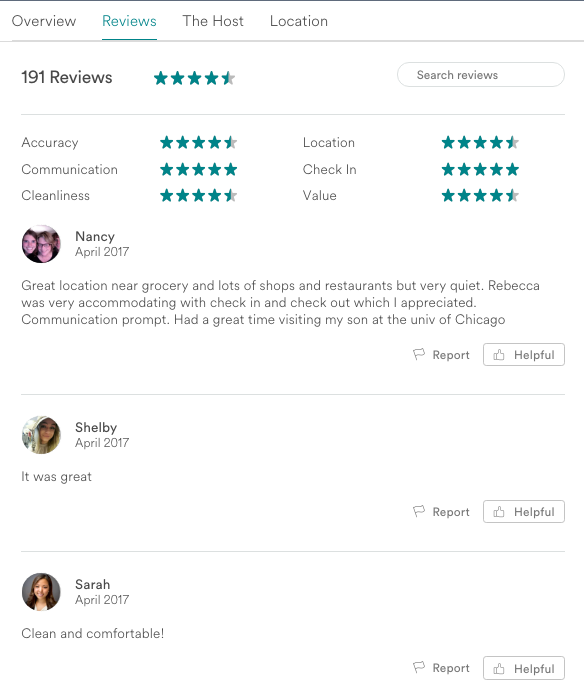
\includegraphics[width=.8\textwidth]{figures/sample3-reviews}
\caption{Sample review information}
\end{figure}
\begin{figure}\centering
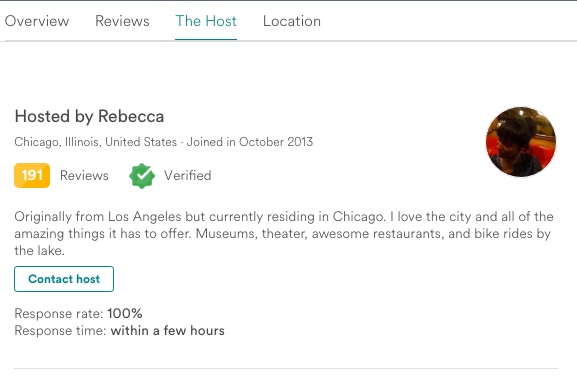
\includegraphics[width=.9\textwidth]{figures/sample4-host}
\caption[Sample host information]{Sample host information available. Note that this Figure reflects the changes made to the website after Airbnb updated its discrimination policy. The guests in my data would have seen a larger host profile picture than shown here.}
\end{figure}
\begin{figure}\centering
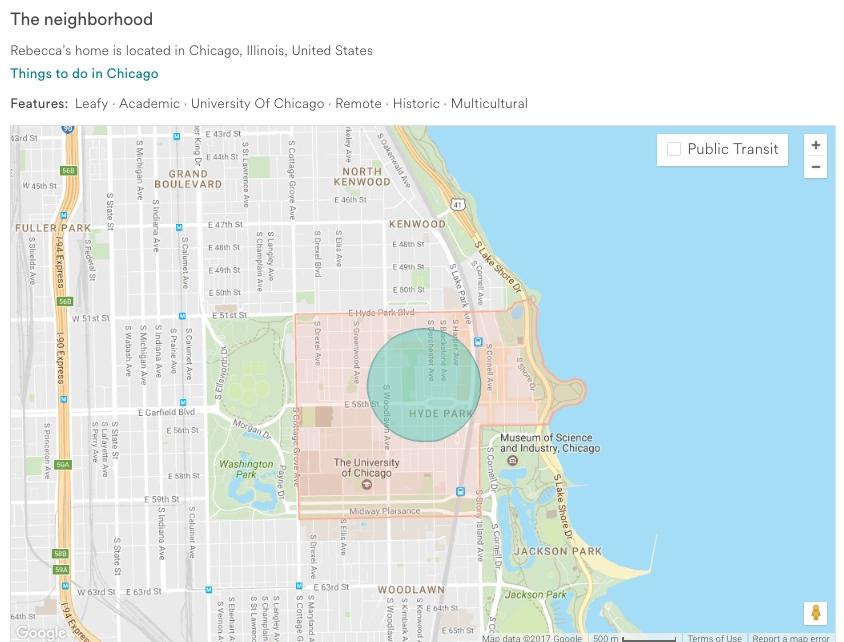
\includegraphics[width=.8\textwidth]{figures/sample5-location}
\caption{Sample location information}
\end{figure}
\begin{figure}\centering
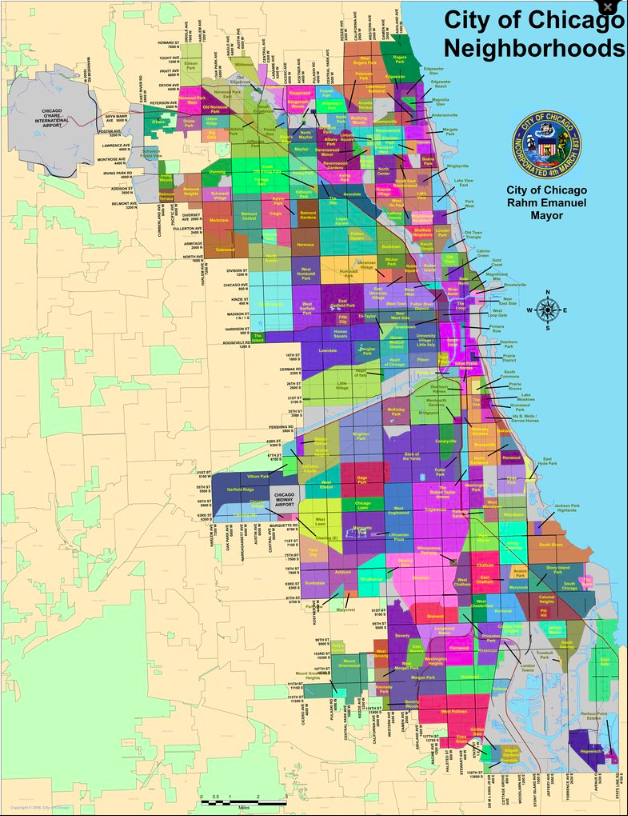
\includegraphics[width=.8\textwidth]{figures/chicago_city_neighborhoods}
\caption[City of Chicago neighborhoods]{City of Chicago neighborhoods, showing level of granularity of neighborhood controls}
\end{figure}



	\label{figures}

\newpage


\begin{comment}
 
***************** TRASH SECTION

Options for first sentence of abstract:
\begin{enumerate}
\item The extent of discrimination on Airbnb, especially against hosts, remains poorly researched. 
\item Despite well-publicized efforts by Airbnb to address discrimination on its platform, the discrimination against hosts remains poorly measured by economists. 
\item Even though discrimination against hosts on Airbnb carries serious economic consequences for agents, the issue has remained poorly researched. 
\item Measuring discrimination is challenging because in the absence of an experiment, it requires controlling for an extensive set of covariates. 
\item Little research has been done on the extent of discrimination against hosts on Airbnb because of data restrictions, and difficulty of setting up an experiment. 
\item This paper leverages the recent rise of sharing economies and the data and standardization their platforms provide to credibly measure discrimination against minority landlords
\item There is little evidence that these price disparities are due to minority hosts choosing to price their listings lower because of differences in their marginal cost, or offering their listing up for rent for shorter periods of time, than white hosts. I also find little evidence that this effect is due to minority hosts owning listings of worse quality.(LAST SENTENCE OF FORMER ABSTRACT)  
\end{enumerate}

In this section, I consider alternative explanations for the price differences I found between minority and white hosts. In particular, I examine three relevant mechanisms that are not discrimination that could explain my results. I will then argue that these mechanisms would be insufficient in doing so. 

\textbf{2. Price observed during the scrape is not the price normally set by hosts or observed by guests}

The prices I used in my data analysis were prices from one particular day in 2015-2016. I ran my regressions on the assumption that this is the price that hosts set and that guests observe that drives guest booking decisions and host revenue outcomes. However, imagine that for one day, all of the white people on Airbnb raise their prices. That day, the scrape happens to take place, and the next day, the prices of White hosts all go back down. Then, the price that I observed in my data for White hosts would be high even though it doesn't incorporate real demand differences between races nor is tied to listing characteristics or host quality. While this may seem like an unlikely scenario, price hikes for the weekend or for holidays like July 4th or New Year's may give rise to a similar situation if black hosts change their prices differently than White hosts. 

TO-DO - Check price time series data to prove that prices don't move around that much during the month/year. 

\textbf{3. Data clean-up disproportionately dropped lower-priced listings of White hosts or higher-priced listings of minority hosts}

During my analysis, I left out hosts that had no profile picture. If hosts are aware of the potential effects of discrimination, minority hosts might be less likely to include a profile picture. If minority hosts who own higher-priced listings dropped out of the data set in this way, my coefficients might be biased downward because the sample doesn't include the higher-priced listings owned by minority hosts. A similar thing could have happened when I restricted my data set to listings with a price per night of less than \$800, and to listings owned by hosts who owned fewer than 20 listings total. If those hosts who owned a lot of listings or charged wildly high prices per night were disproportionately black, Hispanic, or Asian, I'd see a similar downward bias on my coefficients.

TO-DO - Examine who I am dropping when I do data-clean up. 

************Garbage
After controlling for listing characteristics, host characteristics, and the neighborhood location of the Airbnb, and time on the market, I find that all host categories, but especially black male hosts, white female hosts, black female hosts, and Asian female hosts, for whom the result is statistically significant at at least the p < .01 level, earn approximately \$200 less during the course of their listing than white male hosts.  will earn \$190 - \$284 less revenue from their Airbnb over the course of the posting relative to their white male peers. The effect is statistically significant at the p < .001 level for white female and black female hosts, and significant at the p < .01 level for black male hosts and Asian female hosts. While there is a large downward effect on revenue for Hispanic male, Hispanic female, and Asian male hosts, it does not persist after controlling for listing and host characteristics. Contrary to what one would expect from discrimination literature, out of the groups for whom I could measure discrimination, black male fared the least poorly, earning \$190 less than white male hosts over the course of their listing?s lifetime. Women as a whole, regardless of race, do worse than black men. Asian women earn \$232.6 less in revenue and white women earn \$272 less in revenue than white male peers. Black women hosts fare the worst out of any of the groups considered, earning \$283.6 less than white men over the course of their Airbnb listing. 

white male reviewers gave lower reviews only to Asian female, with a .074-unit decrease relative to white male hosts. Black male guests gave white female hosts .207 units, two white male hosts .624 lower, Asian men .517 units higher quality reviews than they gave white men. White females gave lower quality reviews only to Asian women at a rate of .099 units less. Black female reviewers gave Airbnbs owned by two black women an entire valence point, 1.005 units better reviews than white male hosts, but rated Hispanic women .647 units lower. Asian females rated Black male hosts .358 units worse than white male hosts. 


TO-DO: Add Levitt and Fryer? Black names paper
List (2004) found a similar result at baseball card shows, with Black sellers getting offer 3-30\% worse than White sellers. 

Becker explains, ``If someone has a `taste for discrimination', he must act as if he were willing to forfeit income in order to avoid certain transactions; it is necessary to be aware of the emphasis on the words `as if'" (Becker 16).While market discrimination harms the discriminated group because it lowers their wages, taste discrimination can also harm the person discriminating, since they might now be paying more for the same good or service - whether in opportunity cost or price -  because they prefer not to interact with the discriminated group. 
Another type of discrimination laid out by Becker is taste discrimination, in which people ``prefer" not to interact with certain groups. This type of taste discrimination that is based on a general dislike could show up in the reviews that are left on host profiles. If a guest stays with a host against whom they are prejudiced, they may leave a worse review or rating, a shorter review, or no review at all, than a comparable stay with a white host. 

********former introduction

When Dyne Suh was minutes away from arriving at the Airbnb she had booked for a weekend getaway, she received a cancellation notice from the host. Left stranded in a snowstorm, Suh offered to pay extra for her stay. The host, through a series of racist messages on the Airbnb app, revealed that she had cancelled because Suh appeared Asian.\cite{diane}  

This example from February 2017 is an extreme case of overt racism, and ended in Airbnb permanently banning the host from the platform. Yet, over the past several years, users have reported more subtle discrimination on Airbnb through social media stories of hosts cancelling or rejecting guests.\cite{nyt1} After being under fire for most of the year, Airbnb updated its Discrimination Policy in September 2016, increasing instant bookings (the opportunity for guests to book without waiting for host approval) and making host profile pictures smaller.\cite{nyt2} 

Sharing economies platforms create a particularly complex environment for regulating discrimination. On the one hand, agents are constrained by certain features of the user interface - if Airbnb never provided guests with a picture or the name of the host, there would be little opportunity to discriminate. On the other hand, users ultimately have nearly full control of the transactions they engage in. For example, drivers on Uber can choose not to accept certain trips or turn the app on or off at their convenience. 

However, these stories of discrimination against \textit{guests} provide only anecdotal evidence for the larger problem of discrimination in the Airbnb market. The problem of discrimination against \textit{hosts} is not publicized, even though it just as important because it affects the prices, revenues, and sometimes livelihoods of thousands of Airbnb hosts. 
\iffalse %comments out entire section of text
\begin{quotation}
``Suppose there are two groups, designated by $W$ and $N$, with members of $W$ being perfect substitutes in production for members of $N$. In the absence of discrimination and nepotism and if the labor market were perfectly competitive, the equilibrium wage rate of $W$ would equal that of $N$. Discrimination could cause these wage rates to differ; the market discrimination coefficient between $W$ and $N$ [...] is defined as the proportional difference between these wage rates" \end{quotation}
\fi
\end{comment}


\end{document}  